% Options for packages loaded elsewhere
\PassOptionsToPackage{unicode}{hyperref}
\PassOptionsToPackage{hyphens}{url}
\PassOptionsToPackage{dvipsnames,svgnames,x11names}{xcolor}
%
\documentclass[
  12pt,
]{book}
\usepackage{amsmath,amssymb}
\usepackage{lmodern}
\usepackage{setspace}
\usepackage{iftex}
\ifPDFTeX
  \usepackage[T1]{fontenc}
  \usepackage[utf8]{inputenc}
  \usepackage{textcomp} % provide euro and other symbols
\else % if luatex or xetex
  \usepackage{unicode-math}
  \defaultfontfeatures{Scale=MatchLowercase}
  \defaultfontfeatures[\rmfamily]{Ligatures=TeX,Scale=1}
\fi
% Use upquote if available, for straight quotes in verbatim environments
\IfFileExists{upquote.sty}{\usepackage{upquote}}{}
\IfFileExists{microtype.sty}{% use microtype if available
  \usepackage[]{microtype}
  \UseMicrotypeSet[protrusion]{basicmath} % disable protrusion for tt fonts
}{}
\makeatletter
\@ifundefined{KOMAClassName}{% if non-KOMA class
  \IfFileExists{parskip.sty}{%
    \usepackage{parskip}
  }{% else
    \setlength{\parindent}{0pt}
    \setlength{\parskip}{6pt plus 2pt minus 1pt}}
}{% if KOMA class
  \KOMAoptions{parskip=half}}
\makeatother
\usepackage{xcolor}
\usepackage[left=4cm, right=3cm, top=2.5cm, bottom=2.5cm]{geometry}
\usepackage{longtable,booktabs,array}
\usepackage{calc} % for calculating minipage widths
% Correct order of tables after \paragraph or \subparagraph
\usepackage{etoolbox}
\makeatletter
\patchcmd\longtable{\par}{\if@noskipsec\mbox{}\fi\par}{}{}
\makeatother
% Allow footnotes in longtable head/foot
\IfFileExists{footnotehyper.sty}{\usepackage{footnotehyper}}{\usepackage{footnote}}
\makesavenoteenv{longtable}
\usepackage{graphicx}
\makeatletter
\def\maxwidth{\ifdim\Gin@nat@width>\linewidth\linewidth\else\Gin@nat@width\fi}
\def\maxheight{\ifdim\Gin@nat@height>\textheight\textheight\else\Gin@nat@height\fi}
\makeatother
% Scale images if necessary, so that they will not overflow the page
% margins by default, and it is still possible to overwrite the defaults
% using explicit options in \includegraphics[width, height, ...]{}
\setkeys{Gin}{width=\maxwidth,height=\maxheight,keepaspectratio}
% Set default figure placement to htbp
\makeatletter
\def\fps@figure{htbp}
\makeatother
\setlength{\emergencystretch}{3em} % prevent overfull lines
\providecommand{\tightlist}{%
  \setlength{\itemsep}{0pt}\setlength{\parskip}{0pt}}
\setcounter{secnumdepth}{5}
\usepackage[utf8]{inputenc}
\usepackage[spanish,es-tabla]{babel}
\usepackage[fixlanguage]{babelbib}
\usepackage{geometry}
\geometry{letterpaper,left=2cm,top=2cm, right=2cm}
\usepackage{times}           
\usepackage{caption}
\captionsetup[figure, table]{labelfont={bf},labelformat={default},labelsep=period}
\usepackage{graphicx}
\usepackage{booktabs}
\usepackage{longtable}
\usepackage{array}
\usepackage{multirow}
\usepackage{wrapfig}
%\usepackage{float}
\usepackage{colortbl}
\usepackage{xcolor}
\usepackage{pdflscape}
\usepackage{tabu}
\usepackage{threeparttable}
\usepackage{pdfpages}
\usepackage{hyphsubst}
\usepackage{floatrow}
\floatsetup[figure]{capposition=top}
\floatsetup[table]{capposition=top}
\usepackage{booktabs}
\usepackage{longtable}
\usepackage{array}
\usepackage{multirow}
\usepackage{wrapfig}
\usepackage{float}
\usepackage{colortbl}
\usepackage{pdflscape}
\usepackage{tabu}
\usepackage{threeparttable}
\usepackage{threeparttablex}
\usepackage[normalem]{ulem}
\usepackage{makecell}
\usepackage{xcolor}
\ifLuaTeX
  \usepackage{selnolig}  % disable illegal ligatures
\fi
\IfFileExists{bookmark.sty}{\usepackage{bookmark}}{\usepackage{hyperref}}
\IfFileExists{xurl.sty}{\usepackage{xurl}}{} % add URL line breaks if available
\urlstyle{same} % disable monospaced font for URLs
\hypersetup{
  pdftitle={Radiografía del Cambio Social en Chile 2016-2022},
  colorlinks=true,
  linkcolor={blue},
  filecolor={Maroon},
  citecolor={Blue},
  urlcolor={Blue},
  pdfcreator={LaTeX via pandoc}}

\title{Radiografía del Cambio Social en Chile 2016-2022}
\usepackage{etoolbox}
\makeatletter
\providecommand{\subtitle}[1]{% add subtitle to \maketitle
  \apptocmd{\@title}{\par {\large #1 \par}}{}{}
}
\makeatother
\subtitle{Estudio Longitudinal Social de Chile}
\author{}
\date{\vspace{-2.5em}}

\begin{document}
\maketitle

{
\hypersetup{linkcolor=}
\setcounter{tocdepth}{1}
\tableofcontents
}
\listoffigures
\listoftables
\setstretch{1.5}
\hypertarget{introducciuxf3n}{%
\chapter*{Introducción}\label{introducciuxf3n}}
\addcontentsline{toc}{chapter}{Introducción}

El Centro de Estudios de Conflicto y Cohesión Social (\href{https://coes.cl/}{COES}) tiene el agrado de publicar el informe ``Radiografía del Cambio Social'', el cual consolida los principales hallazgos longitudinales de cinco mediciones anuales del Estudio Longitudinal Social de Chile (\href{https://coes.cl/encuesta-panel/}{ELSOC}).

ELSOC es una encuesta desarrollada para analizar longitudinalmente, en un estudio panel, la evolución del conflicto y cohesión social en la sociedad chilena, basándose en modelos conceptuales descritos en la literatura nacional e internacional de las disciplinas del ámbito de la Economía, Sociología, Psicología, Ciencia Política y Estudios Urbanos. Se orienta a examinar los principales antecedentes, factores moderadores y mediadores, así como las principales consecuencias asociadas al desarrollo de distintas formas de sociabilidad en Chile.

Durante los últimos años, Chile se ha visto remecido por importantes eventos que han alterado aspectos sociales, políticos y económicos de la vida nacional: la pandemia asociada al COVID-19, y las consecuencias del estallido social más grande de las últimas décadas, ocurrido a partir de octubre de 2019, el que ha desencadenado un proceso constituyente inédito en la historia de Chile.

Ambos fenómenos han significado un desafío para ELSOC y para la comunidad académica, ya que afecta tanto la forma en que son levantados los datos, como las temáticas que el estudio debe abordar. Sin embargo, ELSOC presenta una oportunidad única: la posibilidad de observar el efecto que éstos fenómenos tienen sobre la población chilena desde una perspectiva longitudinal, analizando el cambio y persistencia de comportamientos, creencias y percepciones presentes en la sociedad.

Este informe se centra en tres aspectos claves de la sociedad chilena que se han visto remecidos en el último tiempo: Política y ciudadanía, donde se exploran temáticas de identificación y participación política, cambios en la relación de la ciudadanía con la política institucional y la justificación de la violencia, entre otros; Salud mental y bienestar, abarcando aspectos de salud mental y bienestar, su relación con la economía y cómo se han visto afectados a raíz de la pandemia; y Cohesión Social, donde se analiza el cambio y estabilidad del conflicto y la cohesión desde una perspectiva territorial, las actitudes y creencias de la ciudadanía en torno a los fenómenos de la migración, del sexismo y la meritocracia; entre otros.

\hypertarget{presentaciuxf3n-del-estudio}{%
\chapter{Presentación del estudio}\label{presentaciuxf3n-del-estudio}}

\hypertarget{sobre-coes}{%
\section{Sobre COES}\label{sobre-coes}}

El Centro de Estudios de Conflicto y Cohesión Social (\href{https://coes.cl/}{COES}) desarrolla investigación colaborativa en temas relacionados al conflicto social y la cohesión (convivencia) en Chile, por medio de un equipo multidisciplinario proveniente de las ciencias sociales y humanidades. COES centra sus actividades académicas y de difusión en el análisis de las múltiples manifestaciones del conflicto y cohesión social en Chile, sus causas, así como también su contexto cultural e histórico.

COES está patrocinado por la Universidad de Chile y la Pontificia Universidad Católica de Chile, y como instituciones asociadas se encuentran la Universidad Diego Portales y la Universidad Adolfo Ibáñez. COES cuenta con el apoyo del Fondo de Financiamiento de Centros de Investigación en Áreas Prioritarias (\href{https://www.conicyt.cl/fondap/sobre-fondap/que-es-fondap/}{FONDAP}, dependiente de la Agencia Nacional de Investigación y Desarrollo (\href{https://www.anid.cl/}{ANID}) del Ministerio de Ciencia, Tecnología, Conocimiento e Innovación (\href{https://www.minciencia.gob.cl/}{MinCiencia}). ELSOC además cuenta como socio al Instituto Milenio para la Investigación en Depresión y Personalidad (\href{https://midap.org/}{MIDAP}).

\hypertarget{sobre-elsoc}{%
\section{Sobre ELSOC}\label{sobre-elsoc}}

\hypertarget{descripciuxf3n-del-estudio}{%
\subsection*{Descripción del estudio}\label{descripciuxf3n-del-estudio}}
\addcontentsline{toc}{subsection}{Descripción del estudio}

El \href{https://coes.cl/encuesta-panel/}{Estudio Longitudinal Social de Chile (ELSOC)} es una encuesta panel, representativa de la población nacional urbana, que analiza la estabilidad y cambio de las creencias, actitudes y percepciones que tenemos los chilenos y chilenas respecto de la convivencia y del conflicto, la cohesión y una amplia gama de aspectos políticos y sociales a lo largo del tiempo.

Este estudio sigue la evolución de cerca de 4.500 chilenos y chilenas a lo largo de una década. Actualmente se encuentran disponibles 5 olas del estudio, abarcando el período entre 2016 y 2022. Sus temas de estudio y su aspecto longitudinal convierten a ELSOC en un recurso único en Chile y América Latina para analizar la evolución de la sociedad chilena y para el desarrollo de las ciencias sociales en Chile.

Durante los últimos años, ELSOC se ha consolidado como un importante insumo para el desarrollo de investigación científica y aplicada en ciencias sociales. En el sitio web de (ELSOC)(\url{https://coes.cl/encuesta-panel/}) se puede acceder a más información sobre el estudio.

\hypertarget{acceso-a-bases-de-datos-elsoc}{%
\subsection*{Acceso a Bases de Datos ELSOC}\label{acceso-a-bases-de-datos-elsoc}}
\addcontentsline{toc}{subsection}{Acceso a Bases de Datos ELSOC}

Las bases de datos y documentación correspondientes se encuentran disponibles, de manera libre y gratuita, en un repositorio de datos, al cual se podrá acceder en el link:

\url{https://dataverse.harvard.edu/dataverse/elsoc}

En este sitio se obtendrá acceso a los datos de las 5 mediciones transversales de ELSOC, así como bases longitudinales que integran las distintas mediciones. En colaboración con el Centro de Inteligencia Territorial (\href{https://cit.uai.cl/}{CIT}), se pone también a disposición las bases ELSOC-CIT. Estas bases de datos permiten combinar la información de ELSOC, y estimaciones e indicadores territoriales y geoespaciales de distinta índole, proveniente de diversas fuentes de información nacional para los períodos 2016 a 2019.

ELSOC tiene un compromiso con los más altos estándares científicos en términos de producción y análisis de datos. Dentro de esta visión global, ELSOC se guía por las principales pautas de Transparencia y Apertura en la investigación científica. Por esta misma razón, los códigos utilizados para el desarrollo de este documento se encontrarán disponibles en \url{https://github.com/edgardo-cerda/reporte-elsoc-2022}.

\hypertarget{caracteruxedsticas-del-diseuxf1o-muestral}{%
\subsection*{Características del diseño muestral}\label{caracteruxedsticas-del-diseuxf1o-muestral}}
\addcontentsline{toc}{subsection}{Características del diseño muestral}

\begin{itemize}
\item
  Unidad de Análisis: Individuos
\item
  Muestra objetivo: 3.000 individuos en muestra original (a partir de 2016) y 1.500 en muestra refresco (a partir de 2018)
\item
  Población Objetivo: Hombres y mujeres de 18 a 75 años, residentes habituales de viviendas particulares ocupadas en zonas urbanas, localizadas en 40 ciudades (92 comunas, 13 regiones) del país
\item
  Periodicidad: Anual.
\item
  Diseño Muestral: Probabilístico, estratificado (por tamaño de ciudades), por conglomerados y multietápico
\item
  Marco Muestral: Marco de muestreo de manzanas del pre-censo 2011
\item
  Unidades de Muestreo: Primero se eligen ciudades (UPM), luego manzanas (USM), y sub-bloques y viviendas (UTM). La unidad final de selección es la persona
\end{itemize}

\textbf{Organismo Ejecutor}: Consultora Stephanie Eckman y Centro de Inteligencia Territorial (CIT) de la Universidad Adolfo Ibáñez

\begin{figure}

{\centering 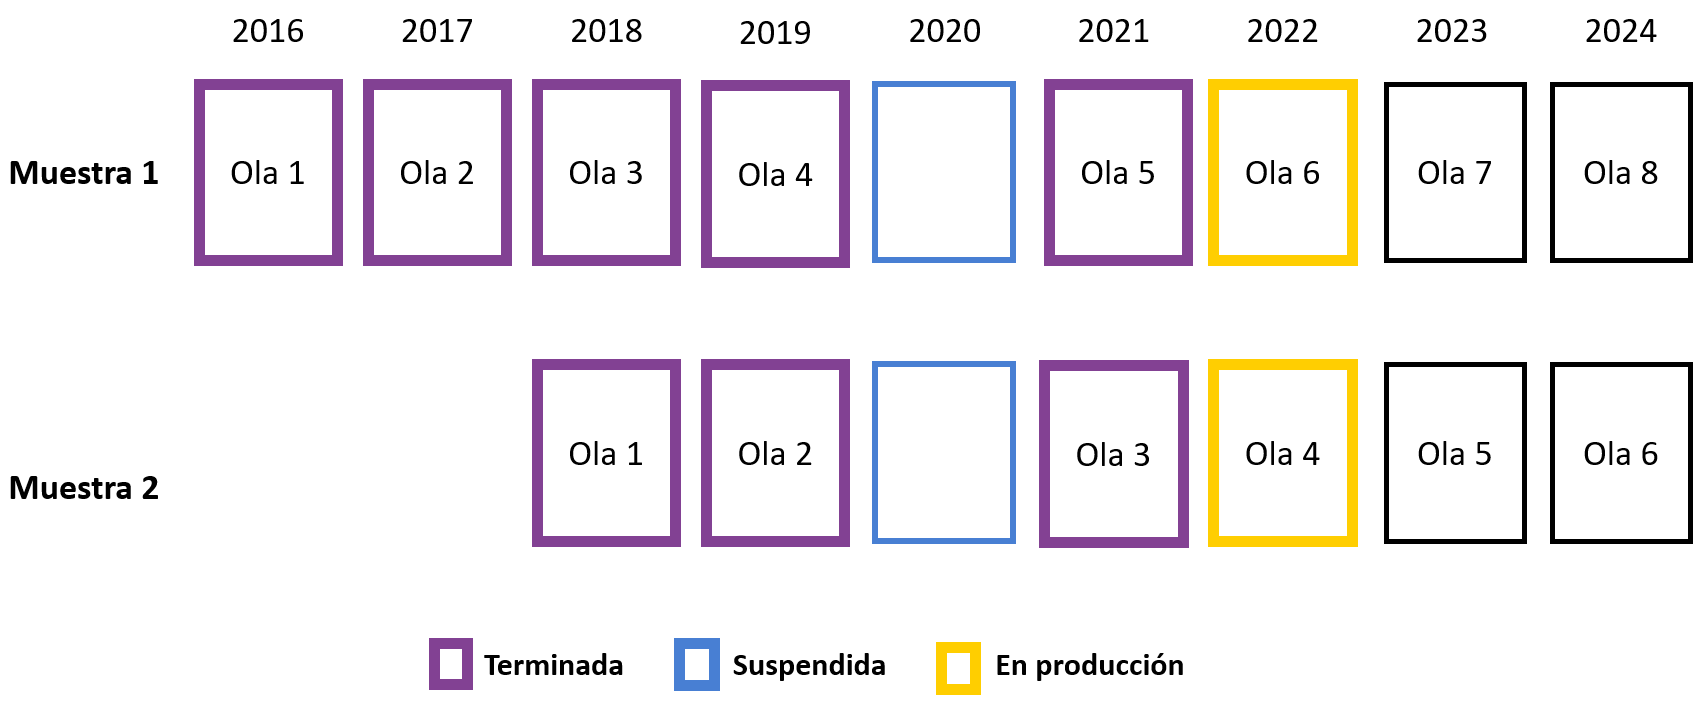
\includegraphics[width=1\linewidth,height=1\textheight]{imagenes/olas_elsoc} 

}

\caption{Mediciones de ELSOC}\label{fig:ilust-olas-elsoc}
\end{figure}

\begin{figure}

{\centering 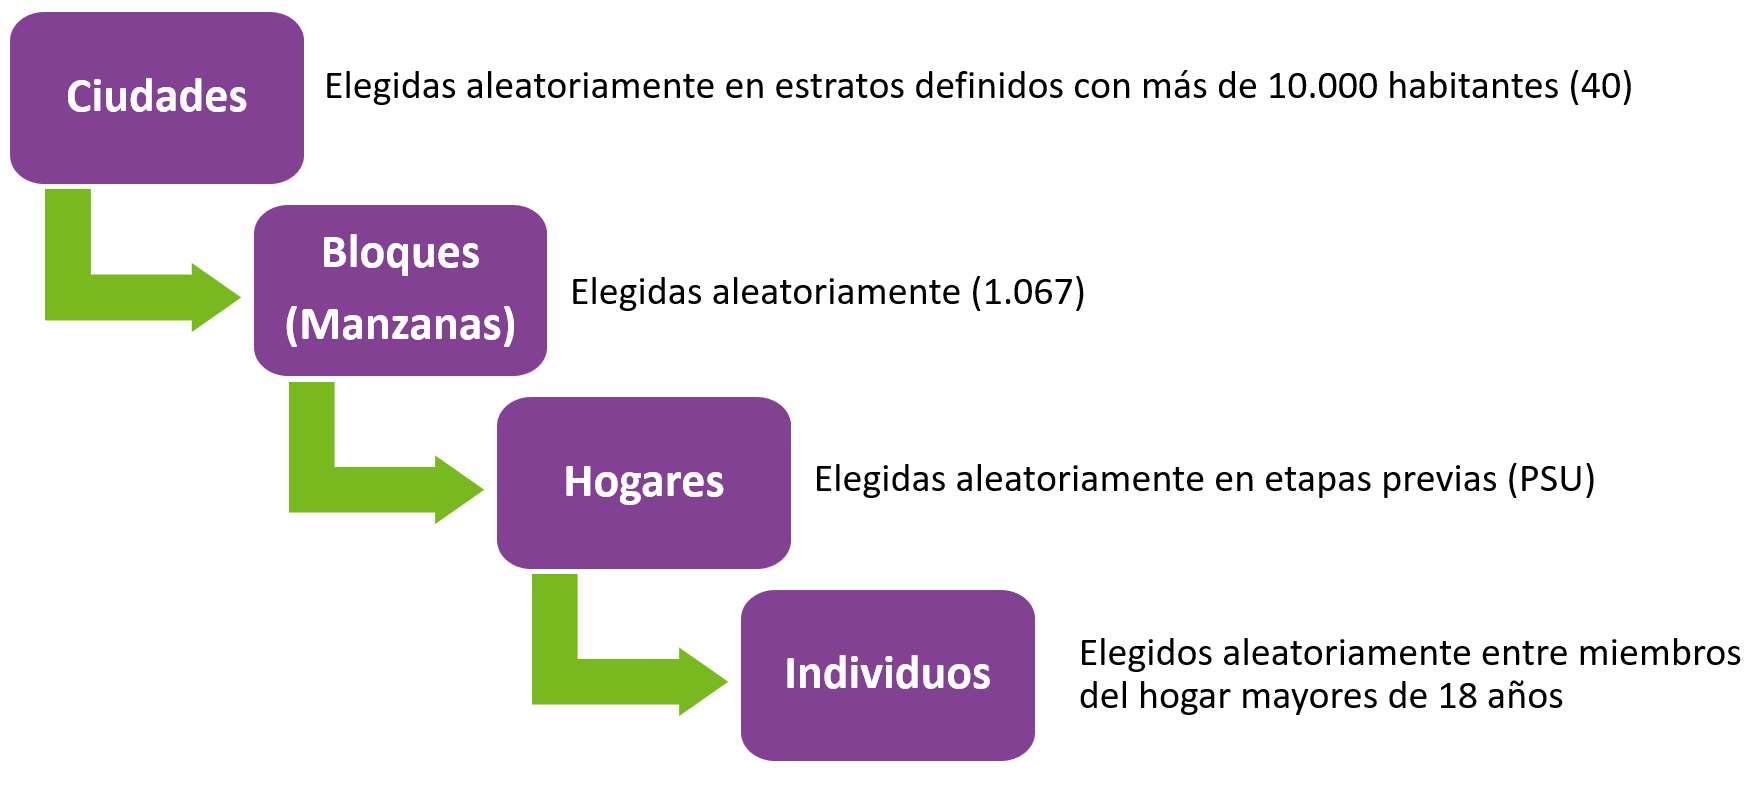
\includegraphics[width=1\linewidth,height=1\textheight]{imagenes/etapas_seleccion} 

}

\caption{Muestreo de ELSOC}\label{fig:ilust-etapas-seleccion}
\end{figure}

\hypertarget{caracteruxedsticas-del-levantamiento-de-datos}{%
\subsection*{Características del levantamiento de datos}\label{caracteruxedsticas-del-levantamiento-de-datos}}
\addcontentsline{toc}{subsection}{Características del levantamiento de datos}

\begin{itemize}
\item
  Formato de aplicación: Cuestionario estructurado. Levantamiento en formato CAPI (Encuesta presencial con asistencia de tablet). Excepcionalmente se cambió a formato CATI (Encuesta telefónica con asistencia de tablet) durante 2022, debido a contingencia COVID-19
\item
  Período de Aplicación: entre Julio y Noviembre de cada año. Debido al estallido social, la cuarta medición se aplicó entre el 21 de noviembre de 2019 y el 9 de marzo de 2020. Debido a la pandemia, la quinta medición se aplicó entre el 29 de enero de 2022 y 12 de julio de 2022
\item
  Instrumento: Cuestionario compuesto por preguntas cerradas de carácter simple y múltiple junto a algunas preguntas abiertas. Combina módulos de preguntas permanentes (medidas en todas las olas) y otras intercaladas entre olas
\item
  Cobertura Temática: Contiene siete módulos temáticos: Territorio, Redes y actitudes sociales, Ciudadanía y democracia, Desigualdad y legitimidad, Conflicto social, Salud y bienestar y Caracterización sociodemográfica
\item
  Incentivos a la participación: Entrega de incentivos monetarios para el encuestado (\$ 6.000 CLP) y de material sobre el estudio (ELSOC y COES). Acciones de seguimiento basadas en la información de contacto (correo electrónico para cumpleaños y días festivos)
\item
  Entrenamiento de entrevistadores: Contratación de entrevistadores con experiencia en encuestas complejas y/o longitudinales. Capacitación centralizada y presencial para coordinadores de campo y un subconjunto de entrevistadores en Santiago (incluidos ejercicios prácticos para la implementación del cuestionario, uso de tabletas y protocolo de contacto). Actividades adicionales en otras regiones de Chile. Diseño de un Manual de entrevistador especializado para el proyecto
\item
  Operaciones de Control y Supervisión: Coordinadores de campo supervisan el trabajo de entrevistadores, verificando el número de visitas, el contacto, la identidad del participante y preguntas claves. Organismo ejecutor realiza una supervisión interna de al menos el 10\% de la muestra (entrevistando nuevamente a algunos encuestados), verificando la duración y la respuesta de los participantes
\end{itemize}

\textbf{Organismo Ejecutor}: Levantamiento a cargo de Centro Micro Datos (CMD) de la Universidad de Chile

\hypertarget{atriciuxf3n-de-la-muestra}{%
\section{Atrición de la muestra}\label{atriciuxf3n-de-la-muestra}}

El diseño de ELSOC contempló entrevistar a 3.000 personas en su muestra original y 1.500 en la muestra refresco. Sin embargo, es habitual que en encuestas panel se reduce el número de participantes, dado que algunos optan voluntariamente por dejar de participar y otras personas no pueden ser recontactadas. Este fenómeno es conocido como atrición, y pueden tener efectos nocivos sobre la utilidad de los datos longitudinales. En el caso de ELSOC, la tasa de atrición es comparativamente baja en comparación a otros estudios similares, por lo que no se considera al momento un problema significativo. A pesar de esto, el año 2018 se introduce una muestra refresco para contrarrestar el efecto de la atrición.

El año 2022, la atrición presenta un alza importante debido a la mayor dificultad que implica el levantamiento durante la pandemia de COVID-19 y al cambio de modalidad.

\begin{table}

\caption{\label{tab:tabla-atricion}Atrición de las muestras de ELSOC entre olas}
\centering
\begin{tabular}[t]{c|c|c|c|c}
\hline
\multicolumn{1}{c|}{ } & \multicolumn{2}{c|}{Muestra original} & \multicolumn{2}{c}{Muestra refresco} \\
\cline{2-3} \cline{4-5}
Medición & Muestra lograda & Atrición & Muestra lograda & Atrición\\
\hline
2016 & 2 928 &  &  & \\
\hline
2017 & 2 474 & 15.5\% &  & \\
\hline
2018 & 2 229 & 9.9\% & 1 519 & \\
\hline
2019 & 2 153 & 3.4\% & 1 264 & 16.8\%\\
\hline
2021 & 1 739 & 19.2\% & 1 001 & 20.8\%\\
\hline
2022 & 1 731 & 0.5\% & 1 001 & 0.0\%\\
\hline
\end{tabular}
\end{table}

\hypertarget{atriciuxf3n-acumulada-seguxfan-sexo-grupo-etuxe1reo-nivel-educacional-y-estrato}{%
\subsection*{Atrición acumulada según Sexo, Grupo etáreo, Nivel educacional y Estrato}\label{atriciuxf3n-acumulada-seguxfan-sexo-grupo-etuxe1reo-nivel-educacional-y-estrato}}
\addcontentsline{toc}{subsection}{Atrición acumulada según Sexo, Grupo etáreo, Nivel educacional y Estrato}

Para el cálculo de atrición acumulada se considera el período 2016-2022 para la muestra original, y el período 2018-2022 para la muestra refresco

\begin{itemize}
\tightlist
\item
  Según sexo:
\end{itemize}

\begin{table}

\caption{\label{tab:tabla-atricion-sexo}Atrición acumulada de ELSOC, según sexo}
\centering
\begin{tabular}[t]{l|c|c|c|c}
\hline
\multicolumn{1}{c|}{ } & \multicolumn{2}{c|}{Muestra lograda en 2022} & \multicolumn{2}{c}{Atrición acumulada} \\
\cline{2-3} \cline{4-5}
Sexo & Muestra original & Muestra refresco & Muestra original & Muestra refresco\\
\hline
Hombre & 612 & 376 & 47\% & 38\%\\
\hline
Mujer & 1 119 & 625 & 37\% & 31\%\\
\hline
\end{tabular}
\end{table}

\begin{itemize}
\tightlist
\item
  Según grupo etáreo:
\end{itemize}

\begin{table}

\caption{\label{tab:tabla-atricion-edad}Atrición acumulada de ELSOC, según grupo etáreo}
\centering
\begin{tabular}[t]{l|c|c|c|c}
\hline
\multicolumn{1}{c|}{ } & \multicolumn{2}{c|}{Muestra lograda en 2022} & \multicolumn{2}{c}{Atrición acumulada} \\
\cline{2-3} \cline{4-5}
Grupo etáreo & Muestra original & Muestra refresco & Muestra original & Muestra refresco\\
\hline
18-29 & 112 & 121 & 78\% & 65\%\\
\hline
30-49 & 584 & 395 & 50\% & 32\%\\
\hline
50-64 & 612 & 310 & 27\% & 26\%\\
\hline
65 o más & 423 & 175 & 0\% & 3\%\\
\hline
\end{tabular}
\end{table}

\begin{itemize}
\tightlist
\item
  Según nivel educacional:
\end{itemize}

\begin{table}

\caption{\label{tab:tabla-atricion-educ}Atrición acumulada de ELSOC, según nivel educacional}
\centering
\begin{tabular}[t]{l|c|c|c|c}
\hline
\multicolumn{1}{c|}{ } & \multicolumn{2}{c|}{Muestra lograda en 2022} & \multicolumn{2}{c}{Atrición acumulada} \\
\cline{2-3} \cline{4-5}
Nivel educacional & Muestra original & Muestra refresco & Muestra original & Muestra refresco\\
\hline
Basica & 390 & 199 & 41\% & 30\%\\
\hline
Media & 749 & 405 & 40\% & 36\%\\
\hline
Tecnica & 265 & 170 & 45\% & 33\%\\
\hline
Universitaria & 324 & 225 & 39\% & 35\%\\
\hline
 & 1 &  &  & \\
\hline
\end{tabular}
\end{table}

\begin{itemize}
\tightlist
\item
  Según estrato:
\end{itemize}

\begin{table}

\caption{\label{tab:tabla-atricion-estrato}Atrición acumulada de ELSOC, según estrato}
\centering
\begin{tabular}[t]{l|c|c|c|c}
\hline
\multicolumn{1}{c|}{ } & \multicolumn{2}{c|}{Muestra lograda en 2022} & \multicolumn{2}{c}{Atrición acumulada} \\
\cline{2-3} \cline{4-5}
Estrato & Muestra original & Muestra refresco & Muestra original & Muestra refresco\\
\hline
Santiago & 407 & 284 & 44\% & 33\%\\
\hline
Valparaíso & 208 & 90 & 45\% & 42\%\\
\hline
Concepción & 242 & 127 & 38\% & 33\%\\
\hline
Ciudades
grandes & 257 & 192 & 37\% & 35\%\\
\hline
Ciudades medianas
o pequeñas & 617 & 306 & 40\% & 33\%\\
\hline
 &  & 2 &  & \\
\hline
\end{tabular}
\end{table}

\hypertarget{foco-en-el-cambio-longitudinal}{%
\section{Foco en el cambio longitudinal}\label{foco-en-el-cambio-longitudinal}}

Radiografía del Cambio Social tiene como objetivo fundamental caracterizar la estabilidad y el cambio en opiniones, actitudes y conductas de los participantes a lo largo del tiempo, enfocándose en distintas dimensiones de la cohesión y conflicto en Chile.

Para el logro de dicho objetivo, el presente reporte se centrará en un subconjunto de participantes del estudio: los 1.513 entrevistados y entrevistadas que participaron en las cinco olas de ELSOC (por lo tanto, todos son parte de la muestra original). Dicha submuestra será la base empírica de los hallazgos expuestos en las siguientes secciones.

A continuación se describe a este grupo de participantes según los mismos atributos sociodemográficos (sexo, edad, educación y zona de residencia).

Los resultados presentados a continuación incorporan el diseño muestral complejo de la encuesta, por lo que incorporan los ponderadores muestrales ajustados a población regional y sexo, según estrato y conglomerado muestral.

\begin{figure}

{\centering 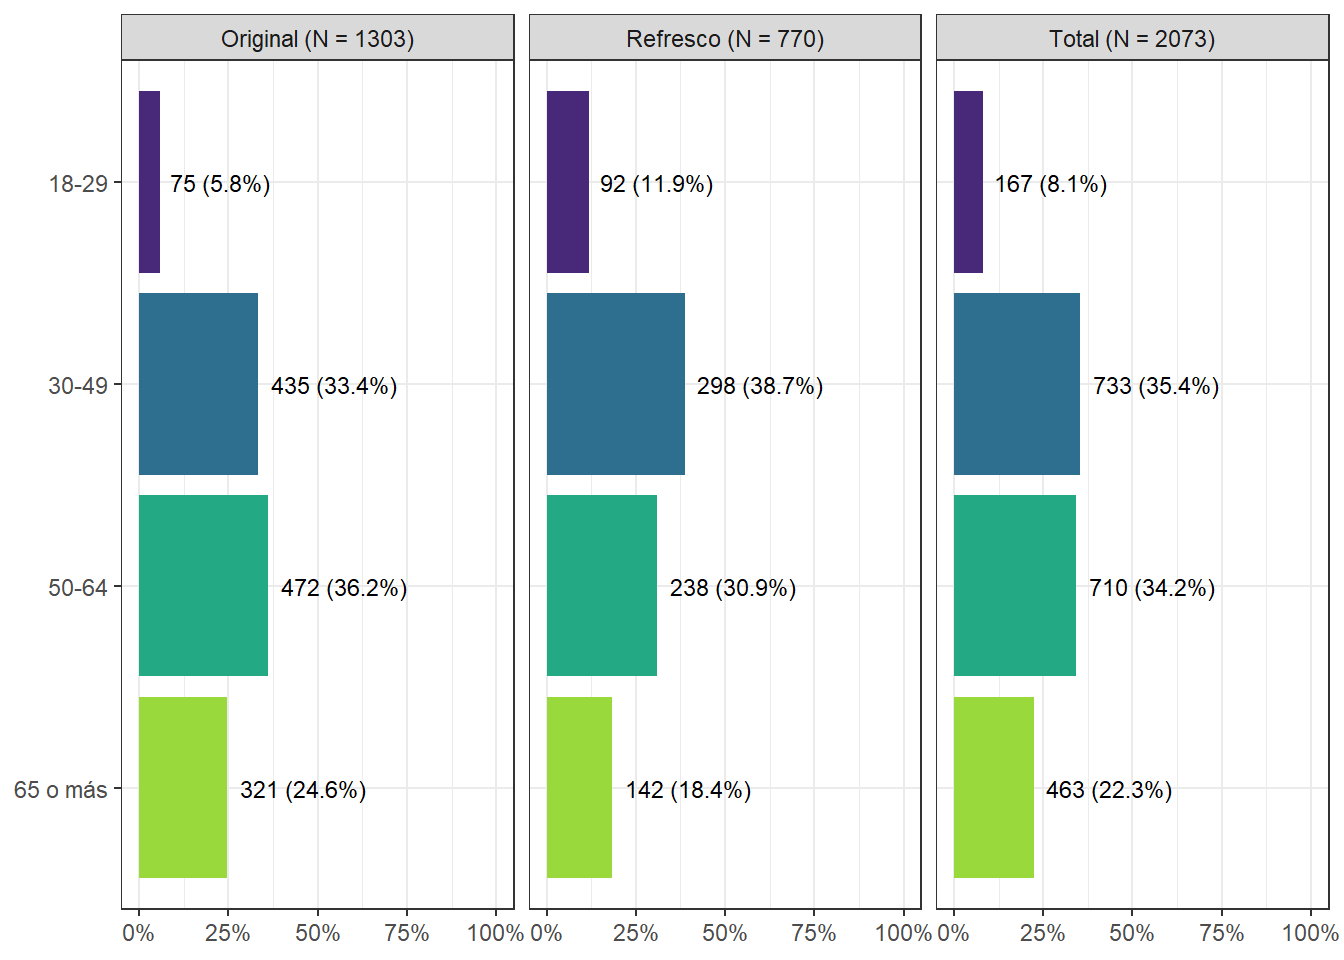
\includegraphics{reporte-elsoc_files/figure-latex/graf-edadt-muestra-1} 

}

\caption{Composición de muestra longitudinal: Tramo Edad}\label{fig:graf-edadt-muestra}
\end{figure}

\begin{figure}

{\centering 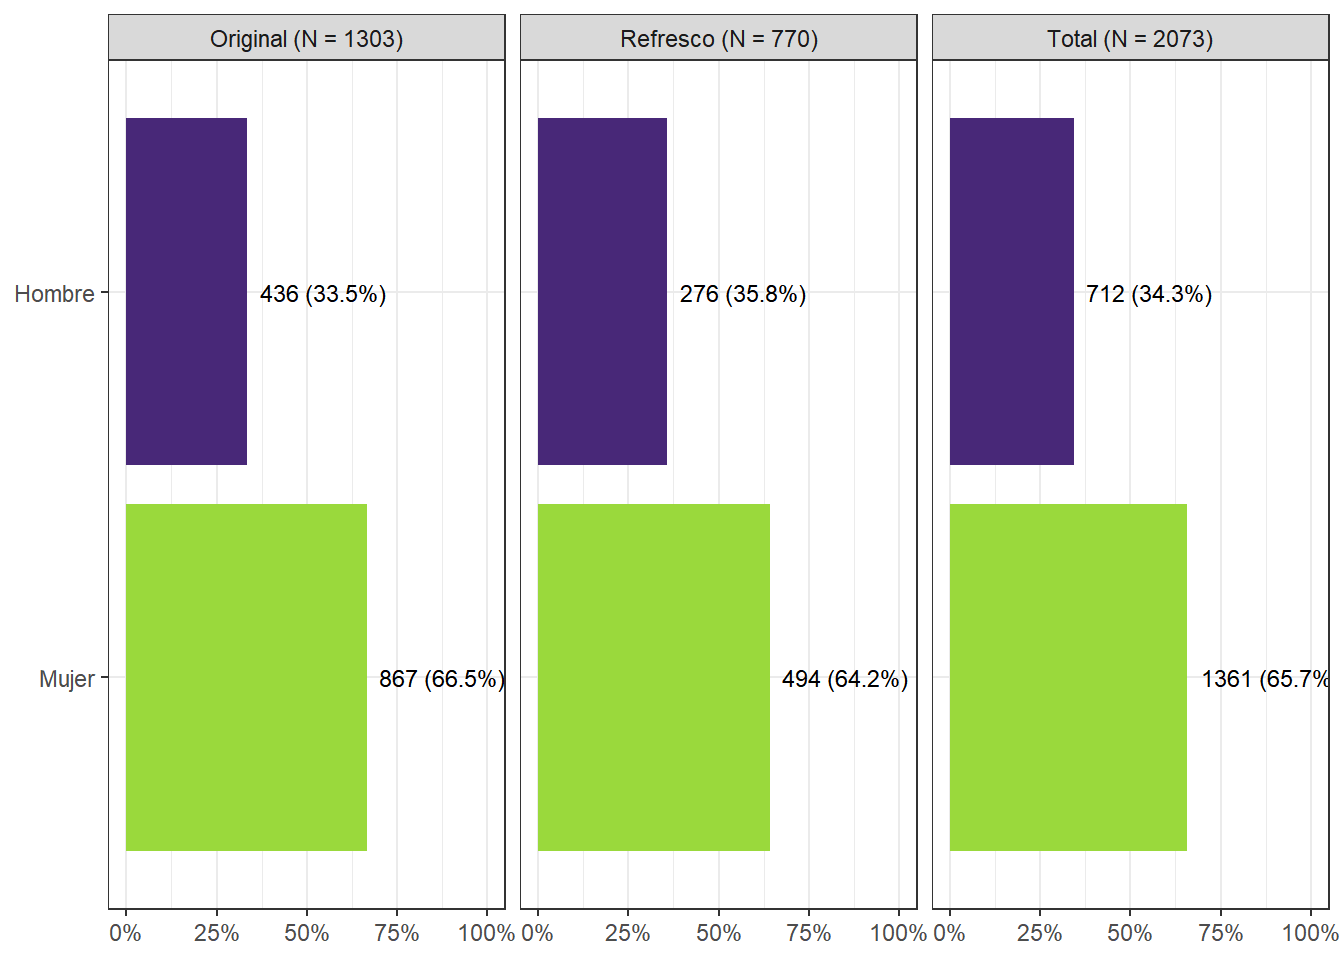
\includegraphics{reporte-elsoc_files/figure-latex/graf-sexo-muestra-1} 

}

\caption{Composición de muestra longitudinal: Sexo}\label{fig:graf-sexo-muestra}
\end{figure}

\begin{figure}

{\centering 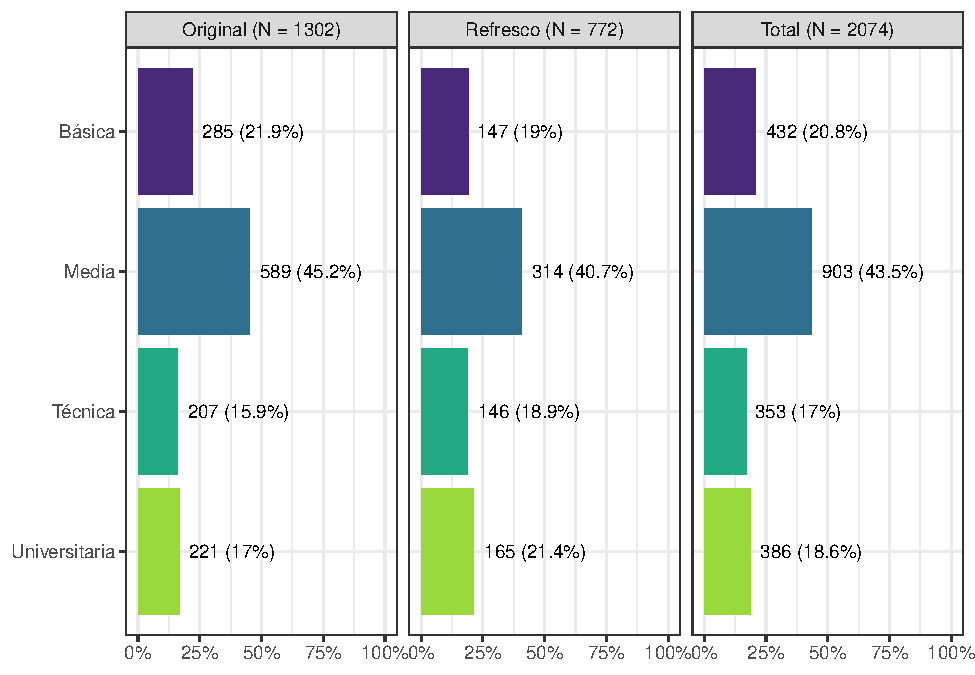
\includegraphics{reporte-elsoc_files/figure-latex/graf-educ-muestra-1} 

}

\caption{Composición de muestra longitudinal: Nivel Educacional}\label{fig:graf-educ-muestra}
\end{figure}

\begin{figure}

{\centering 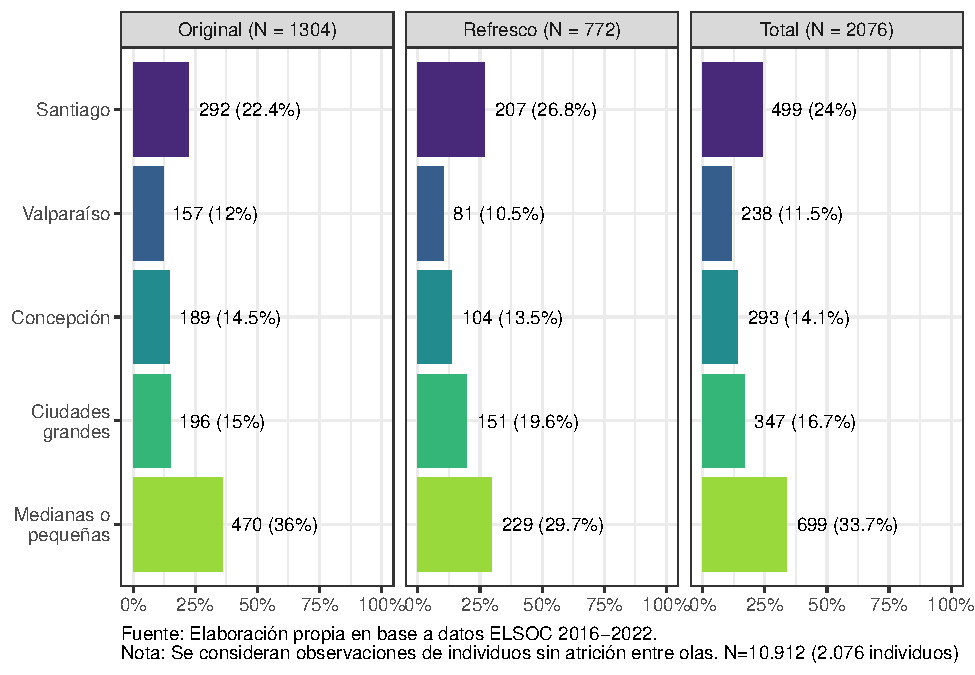
\includegraphics{reporte-elsoc_files/figure-latex/graf-estrato-muestra-1} 

}

\caption{Composición de muestra longitudinal: Estrato}\label{fig:graf-estrato-muestra}
\end{figure}

\begin{figure}

{\centering 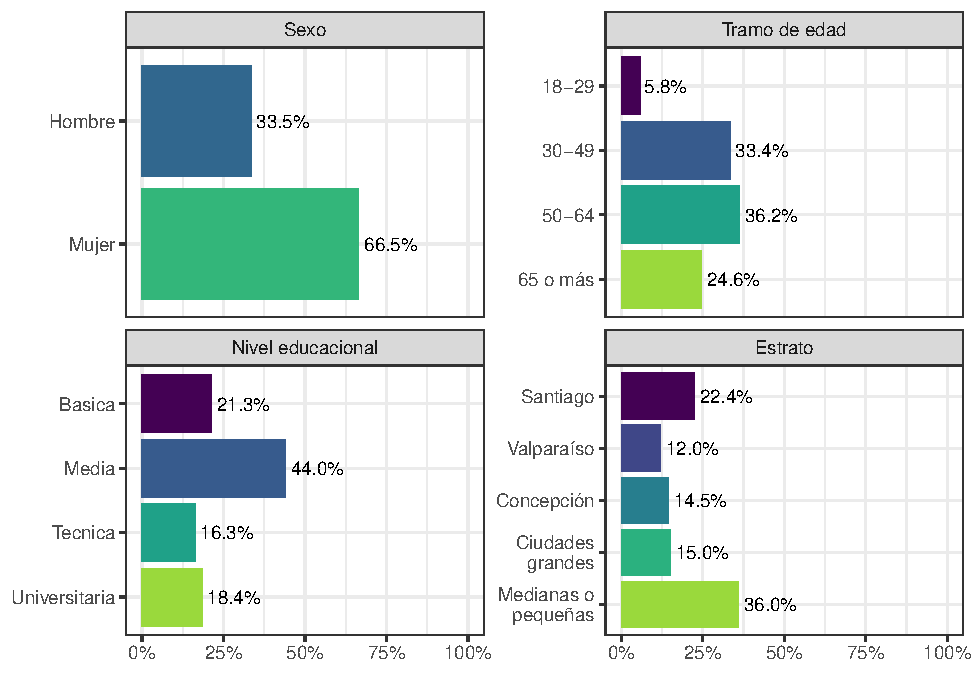
\includegraphics{reporte-elsoc_files/figure-latex/graf-composicion-muestra-1} 

}

\caption{Composición de muestra longitudinal}\label{fig:graf-composicion-muestra}
\end{figure}

\hypertarget{transformaciones-poluxedticas}{%
\chapter{Transformaciones políticas}\label{transformaciones-poluxedticas}}

\hypertarget{participaciuxf3n-electoral}{%
\section{Participación electoral}\label{participaciuxf3n-electoral}}

\begin{center}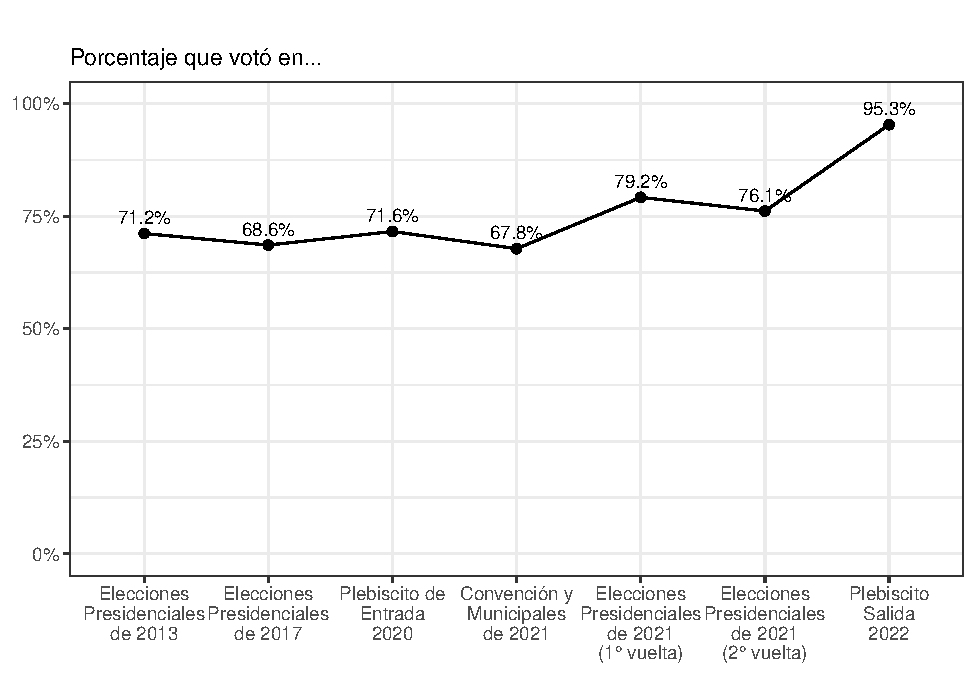
\includegraphics{reporte-elsoc_files/figure-latex/graf-participacion-1} \end{center}

\begin{center}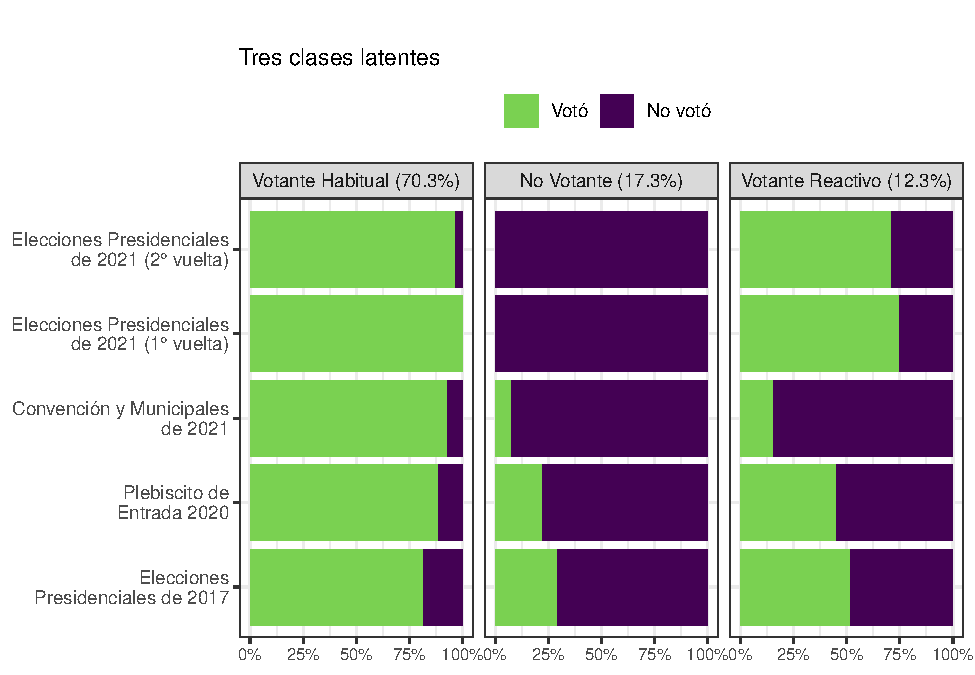
\includegraphics{reporte-elsoc_files/figure-latex/graf-perfiles-3-1} \end{center}

\begin{center}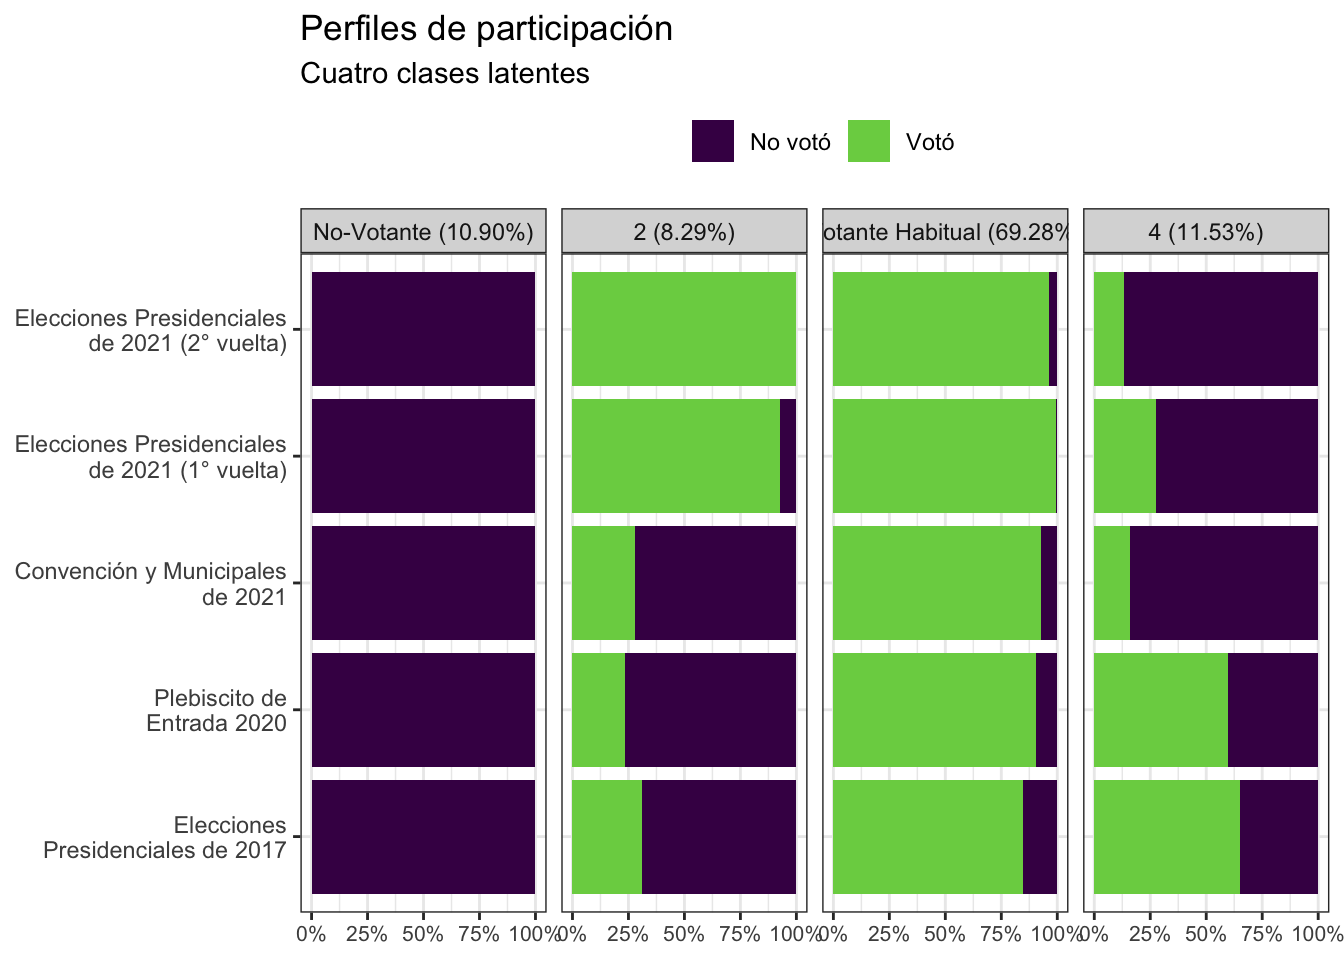
\includegraphics{reporte-elsoc_files/figure-latex/graf-perfiles-4-1} \end{center}

\begin{center}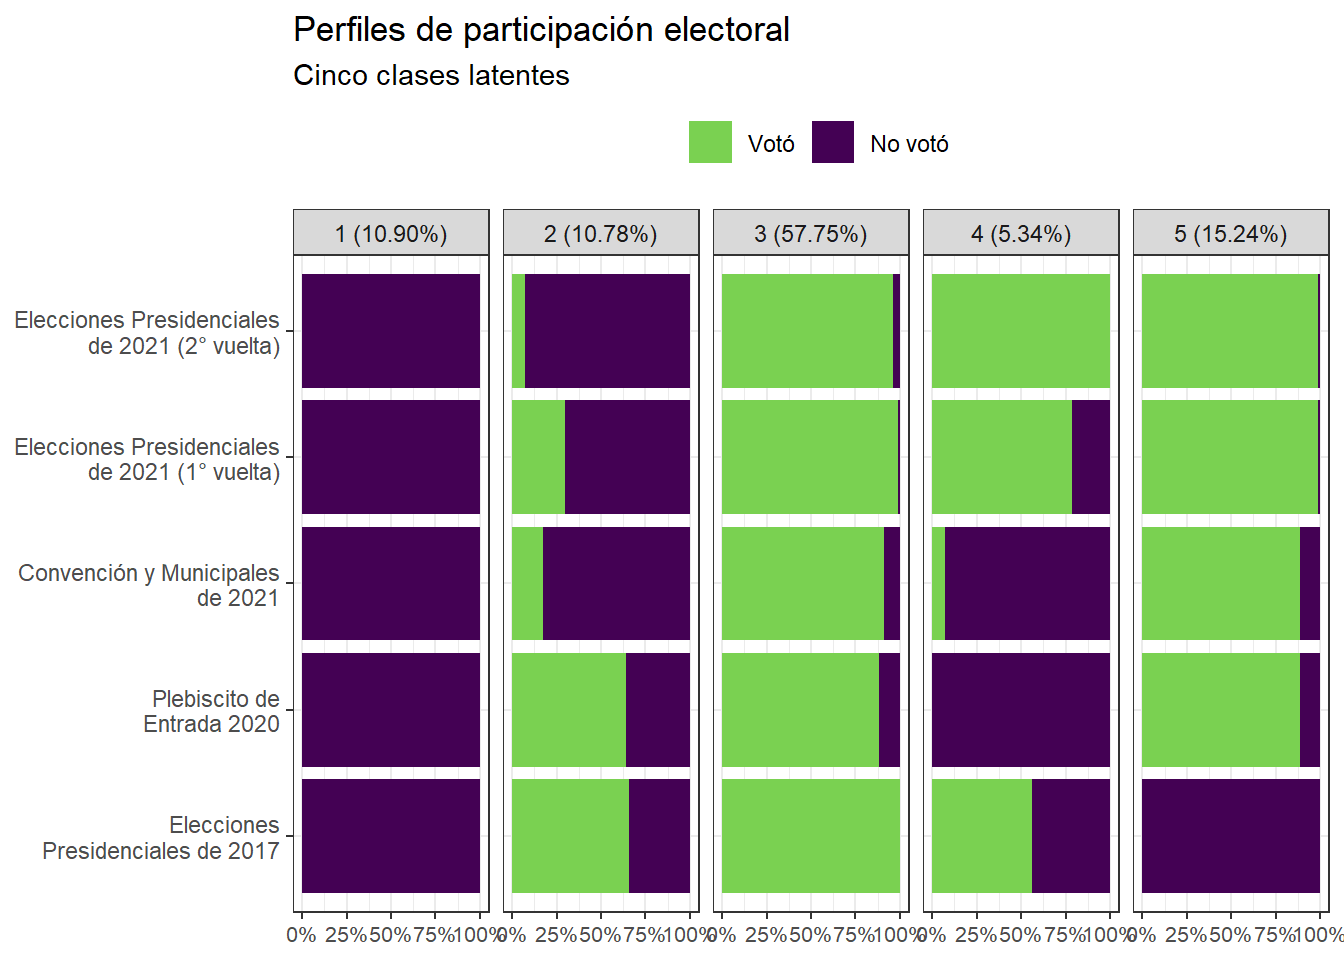
\includegraphics{reporte-elsoc_files/figure-latex/graf-perfiles-5-1} \end{center}

\begin{center}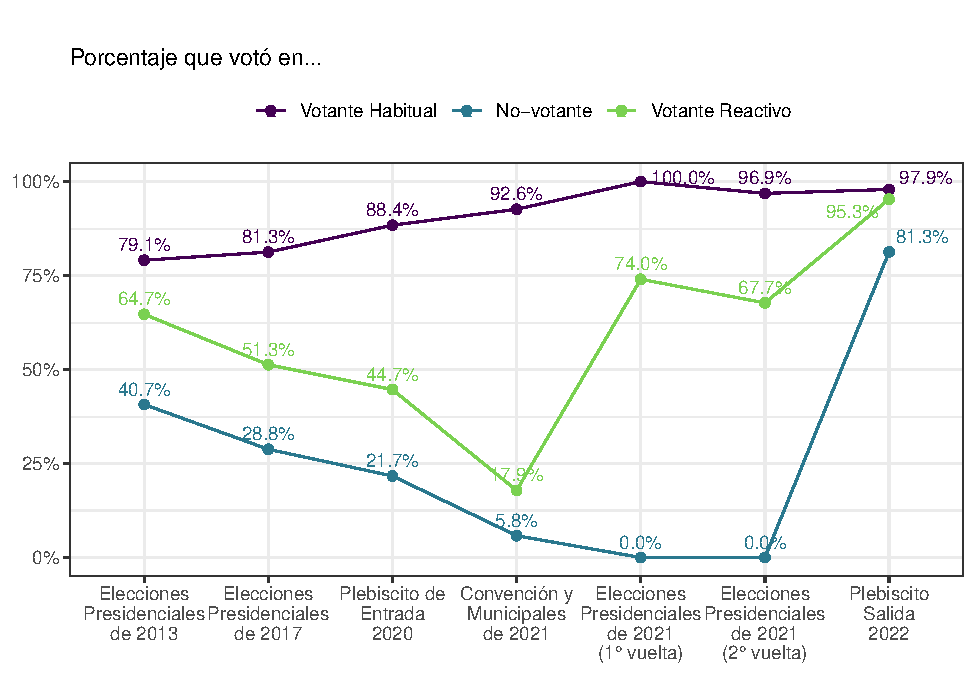
\includegraphics{reporte-elsoc_files/figure-latex/graf-tipo-participacion-1} \end{center}

\hypertarget{caracterizaciuxf3n-del-tipo-de-votante}{%
\section{Caracterización del tipo de votante}\label{caracterizaciuxf3n-del-tipo-de-votante}}

\begin{center}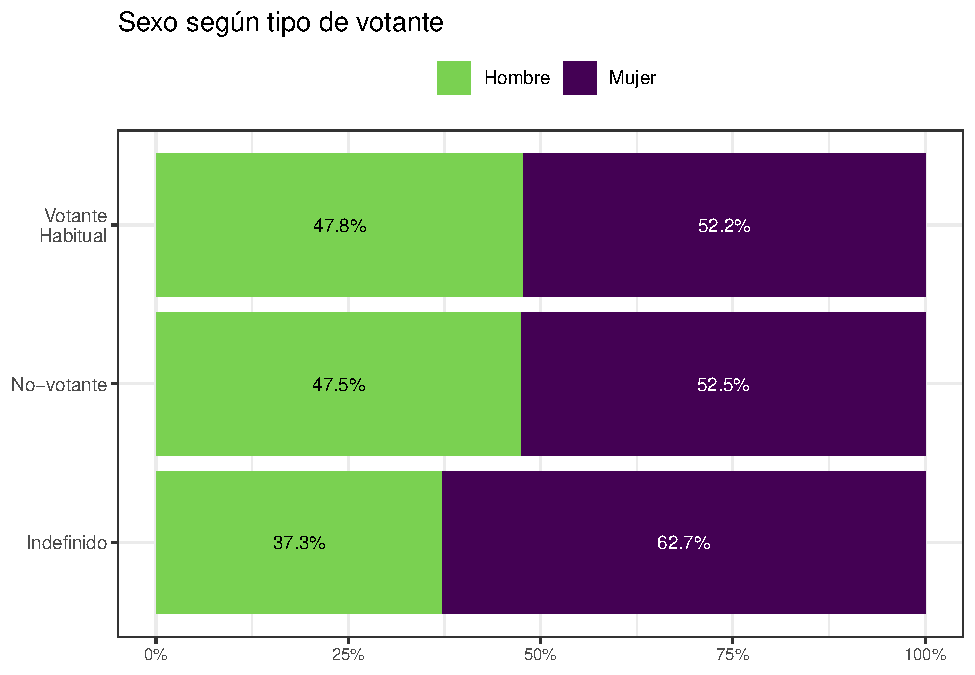
\includegraphics{reporte-elsoc_files/figure-latex/graf-sexo-2-1} \end{center}

\begin{center}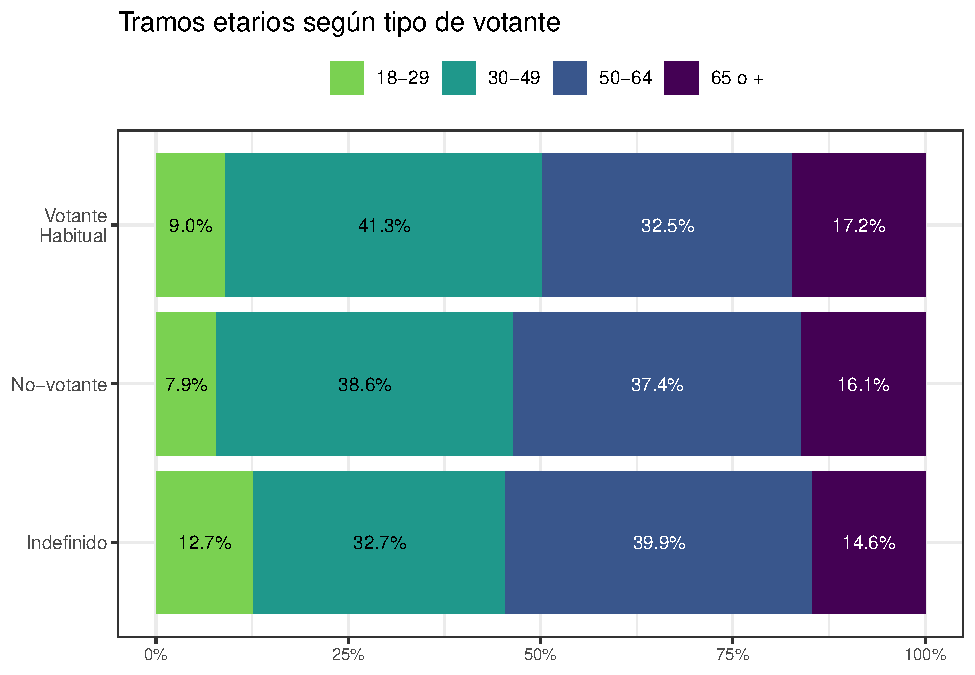
\includegraphics{reporte-elsoc_files/figure-latex/graf-edad-2-1} \end{center}

\begin{center}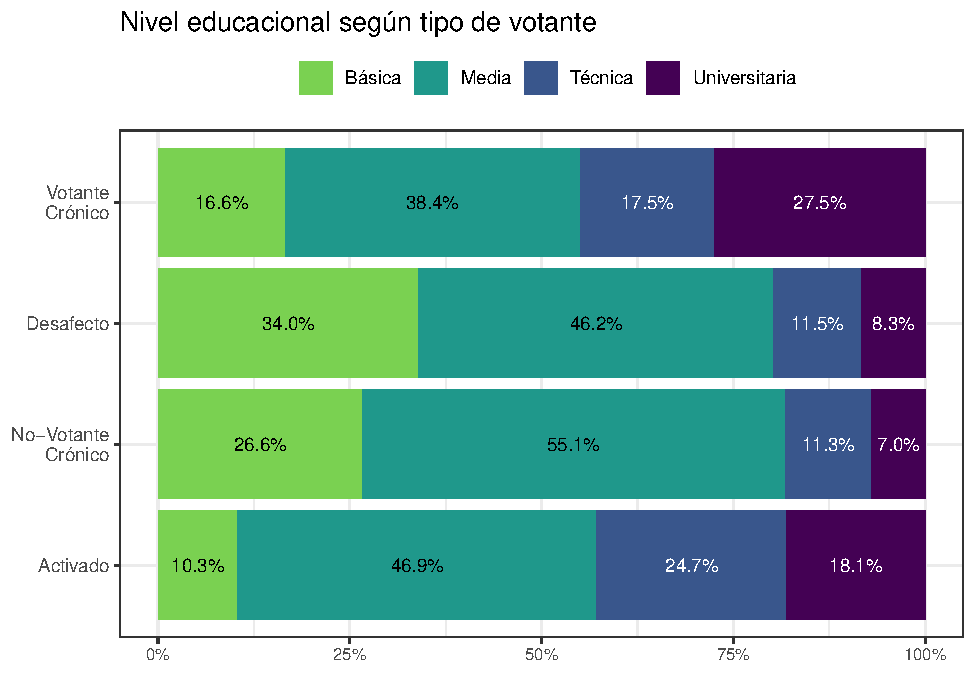
\includegraphics{reporte-elsoc_files/figure-latex/graf-educacion-2-1} \end{center}

\begin{center}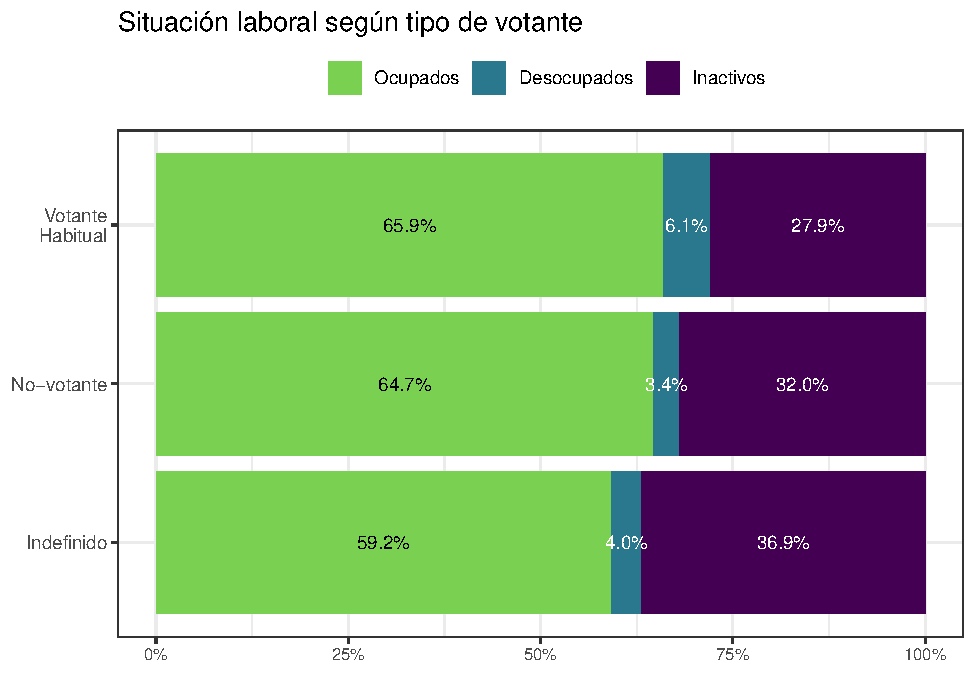
\includegraphics{reporte-elsoc_files/figure-latex/graf-laboral-1} \end{center}

\begin{center}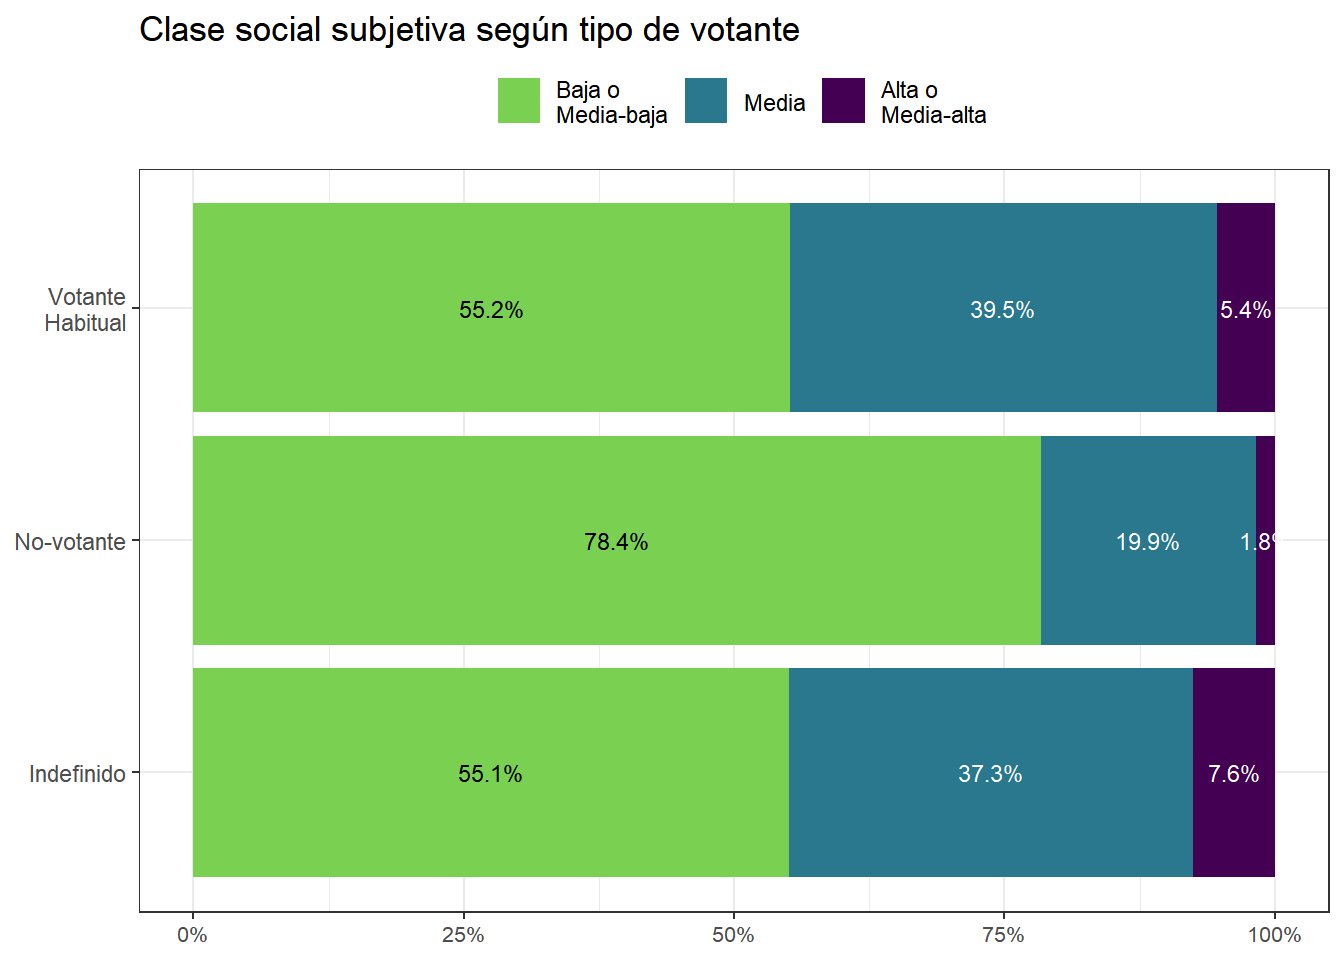
\includegraphics{reporte-elsoc_files/figure-latex/graf-clase-1} \end{center}

\begin{center}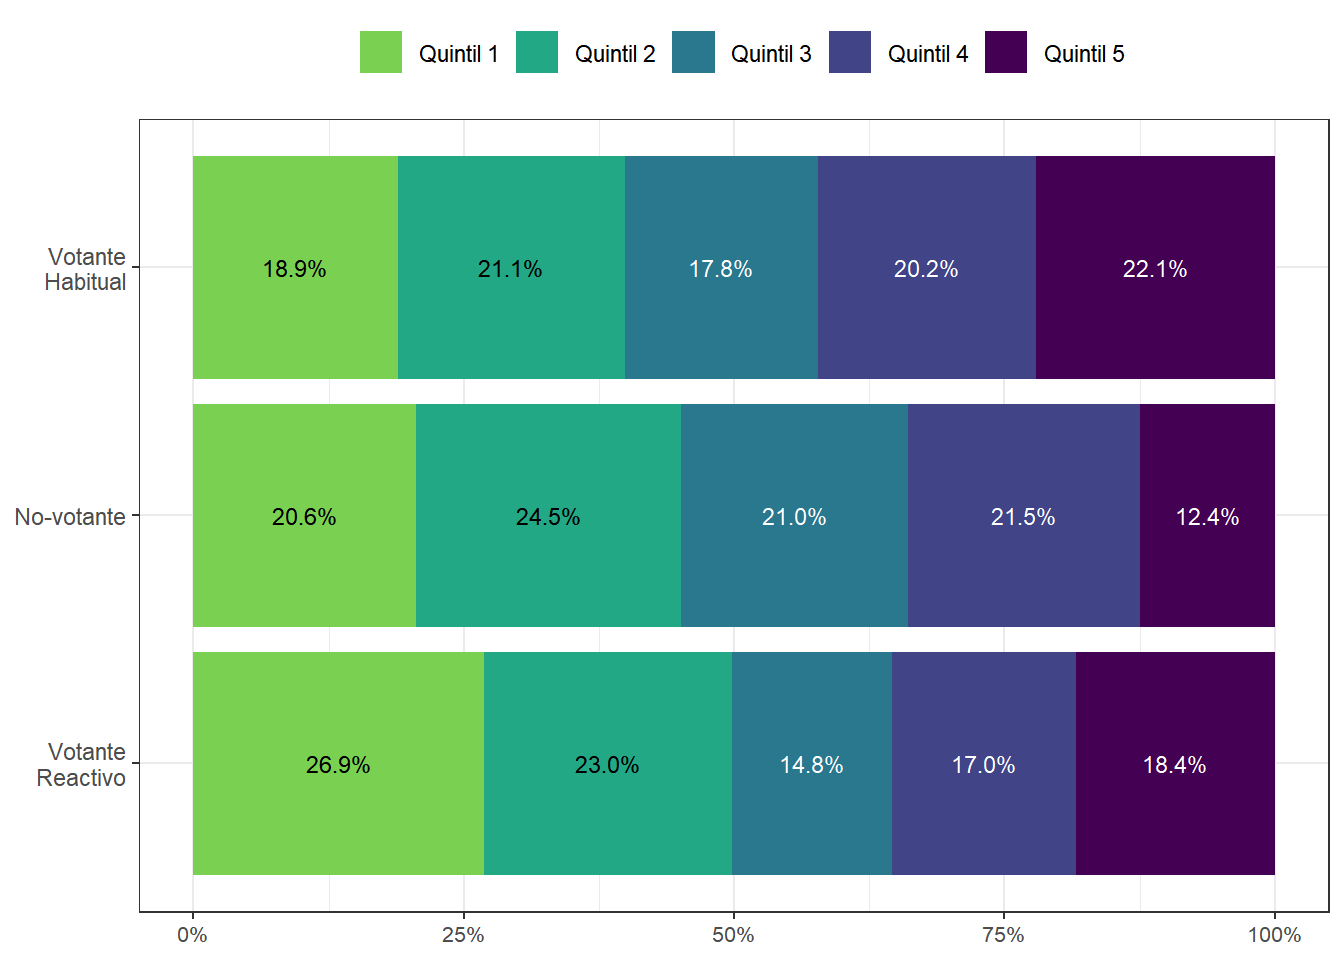
\includegraphics{reporte-elsoc_files/figure-latex/graf-quintil-1} \end{center}

Clase social según deciles de ingreso: deciles 1-4 = Clase baja, deciles 5-9 = Clase media, decil 10 = clase alta.

\begin{center}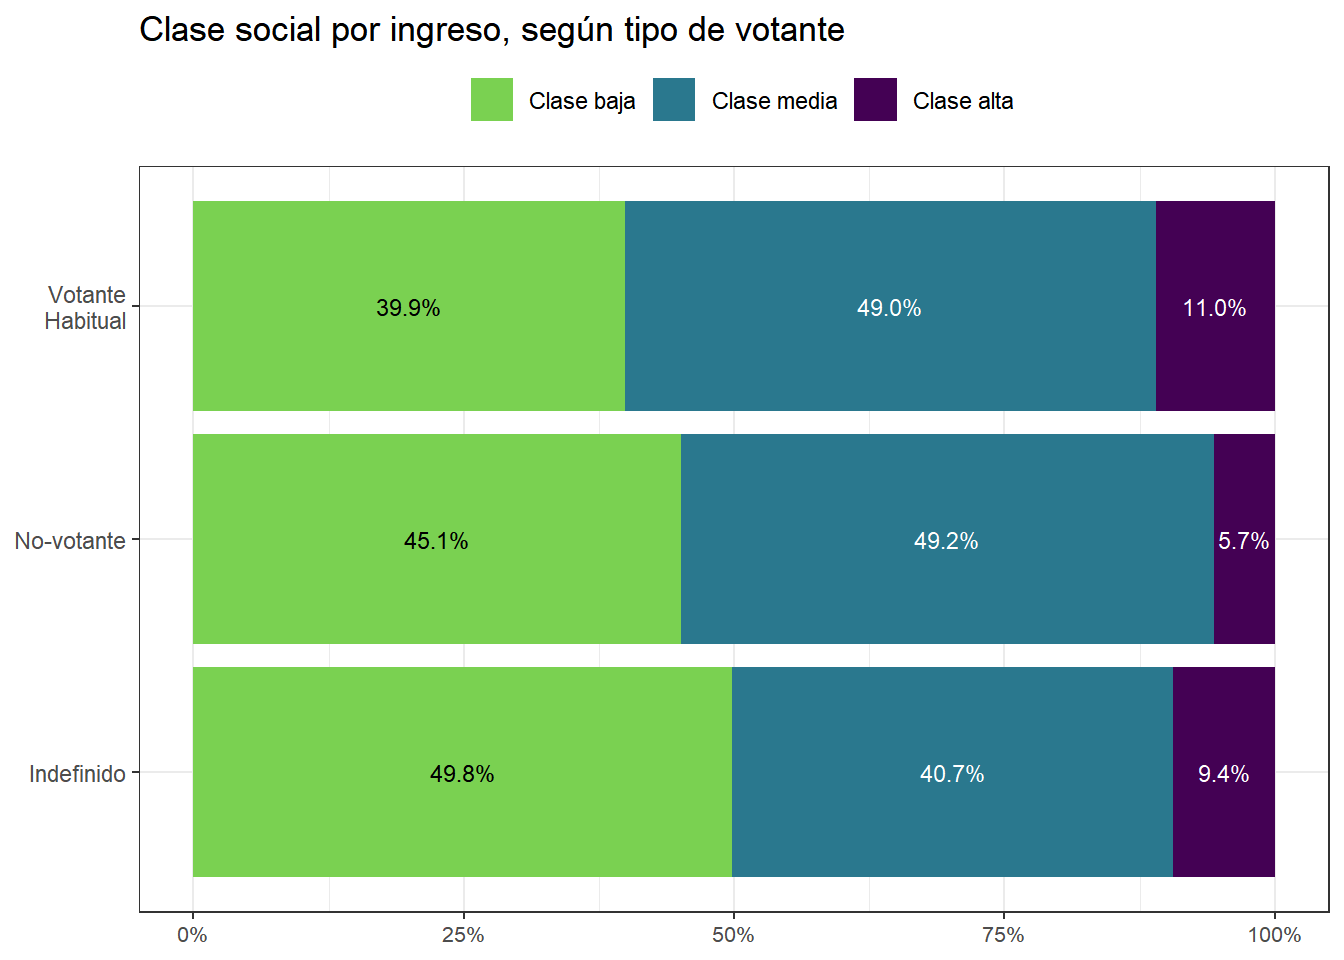
\includegraphics{reporte-elsoc_files/figure-latex/graf-clase-ingreso-1} \end{center}

\hypertarget{proceso-constituyente}{%
\section{Proceso constituyente}\label{proceso-constituyente}}

\begin{center}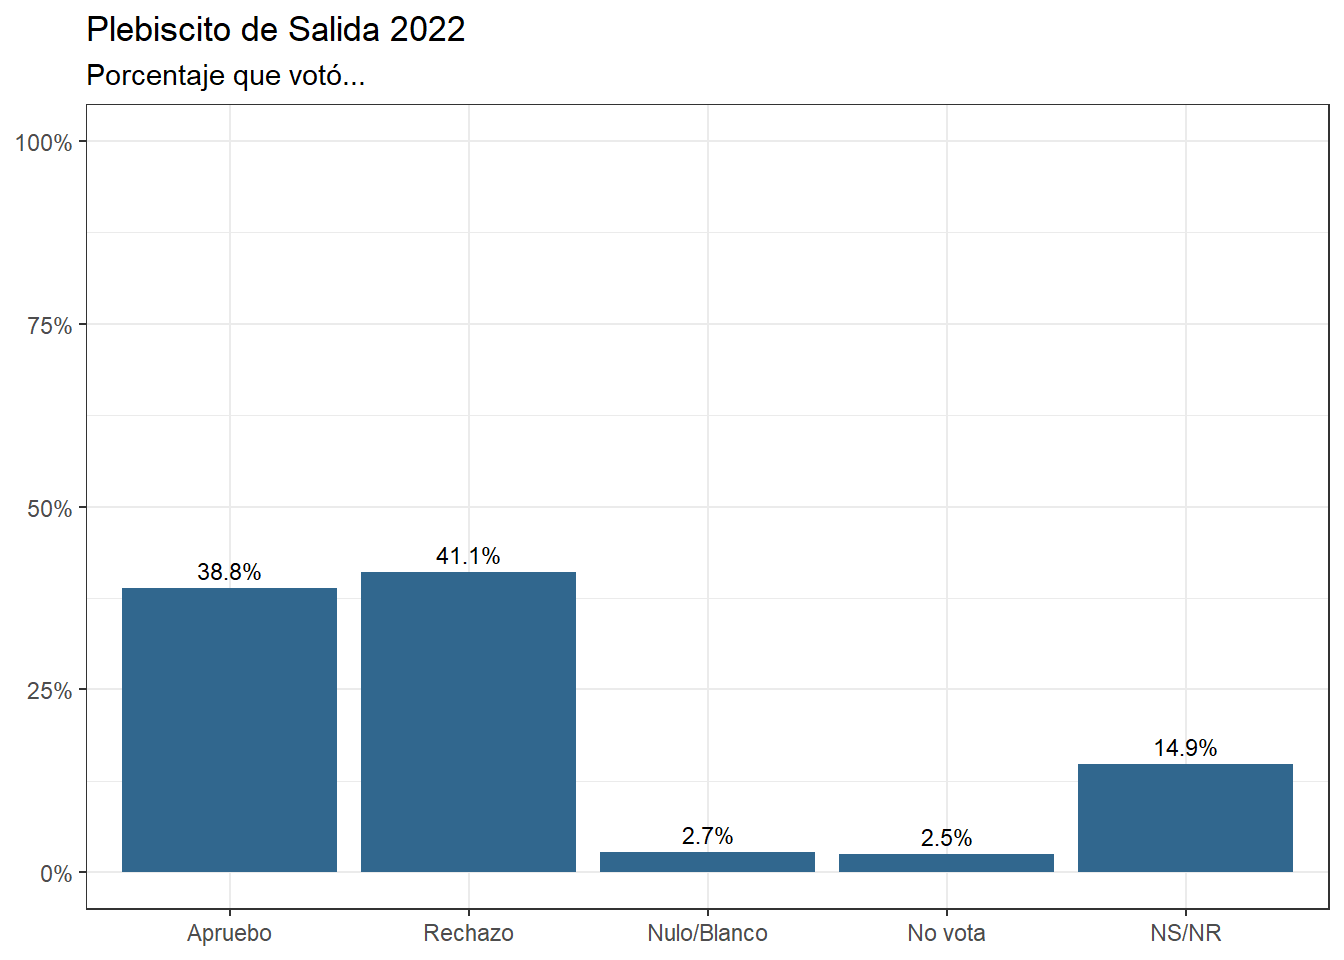
\includegraphics{reporte-elsoc_files/figure-latex/graf-pleb-salida-1} \end{center}

\begin{center}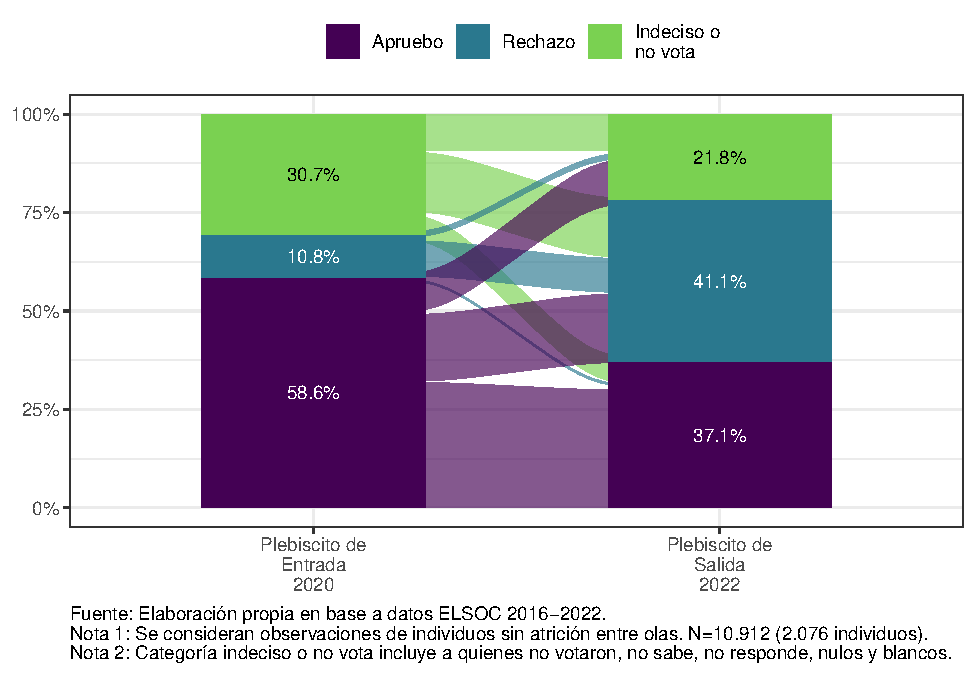
\includegraphics{reporte-elsoc_files/figure-latex/graf-alluvial-pleb-1} \end{center}

\begin{center}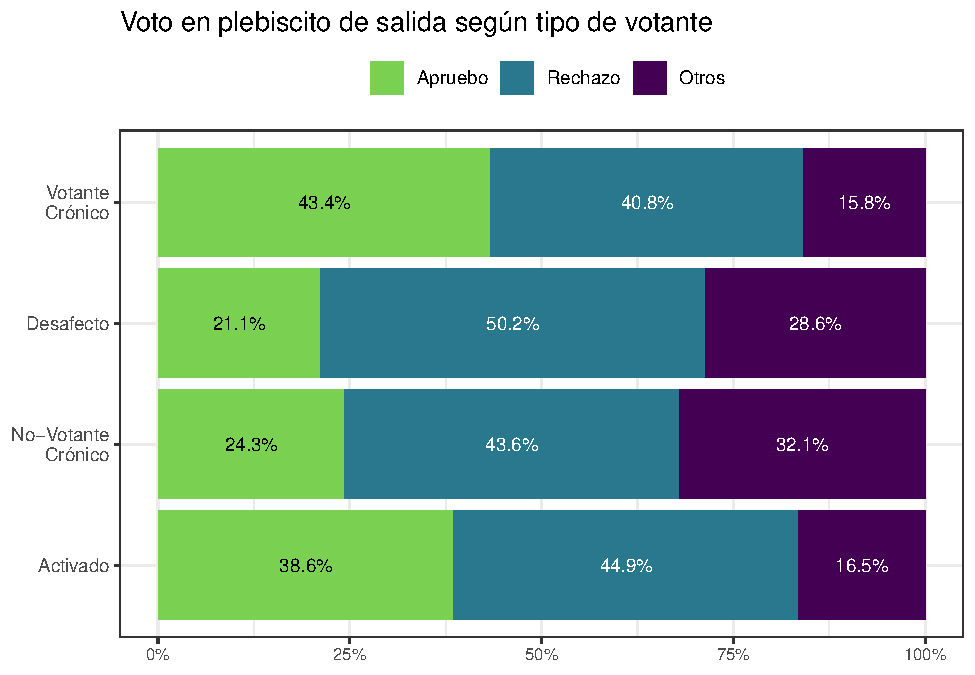
\includegraphics{reporte-elsoc_files/figure-latex/graf-tipo-salida-1} \end{center}

\begin{center}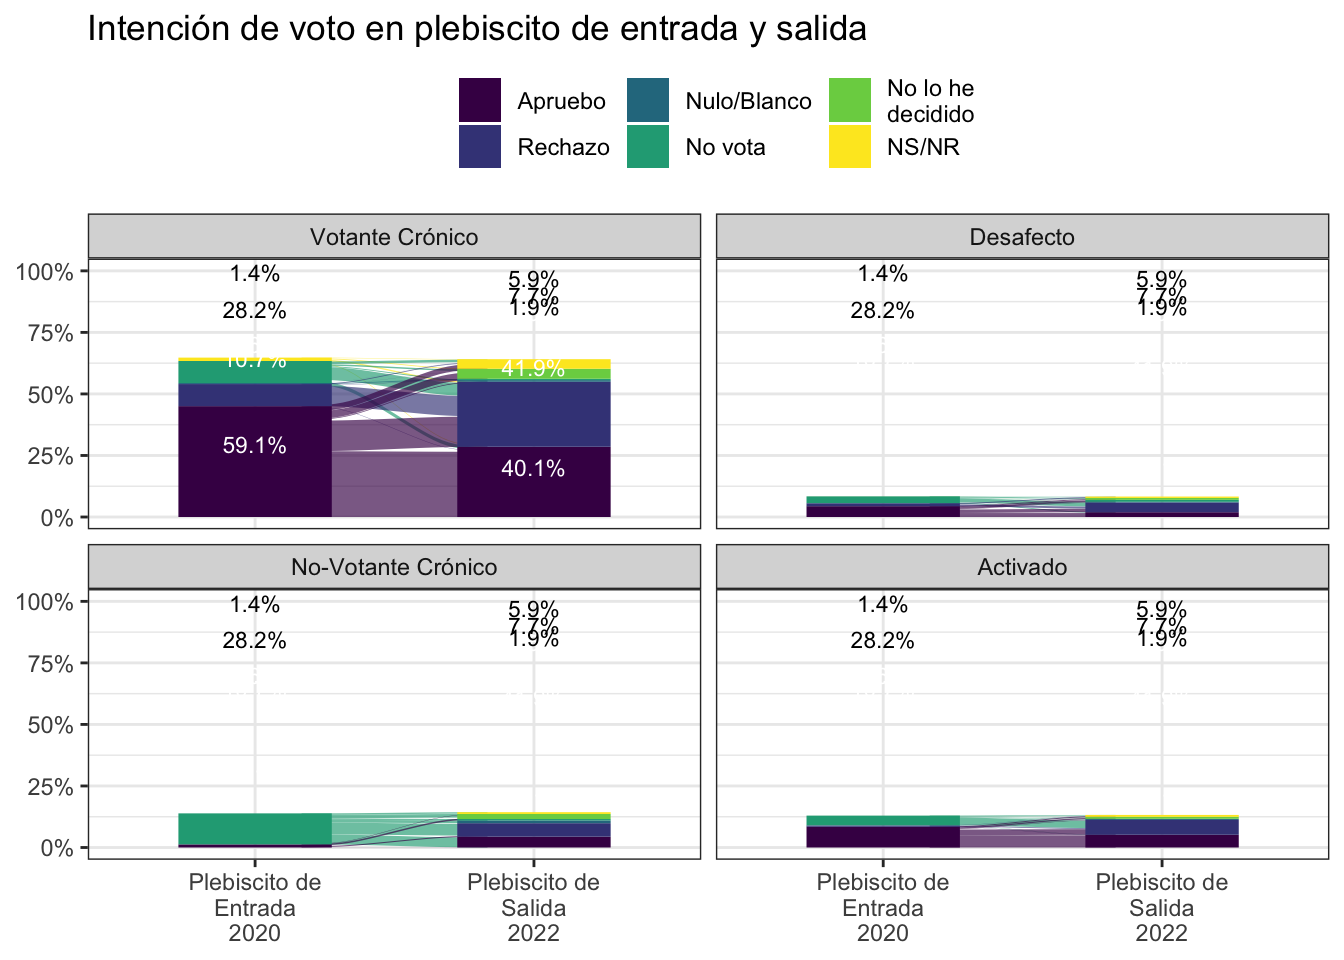
\includegraphics{reporte-elsoc_files/figure-latex/graf-alluvial-pleb-tipo-1} \end{center}

\begin{center}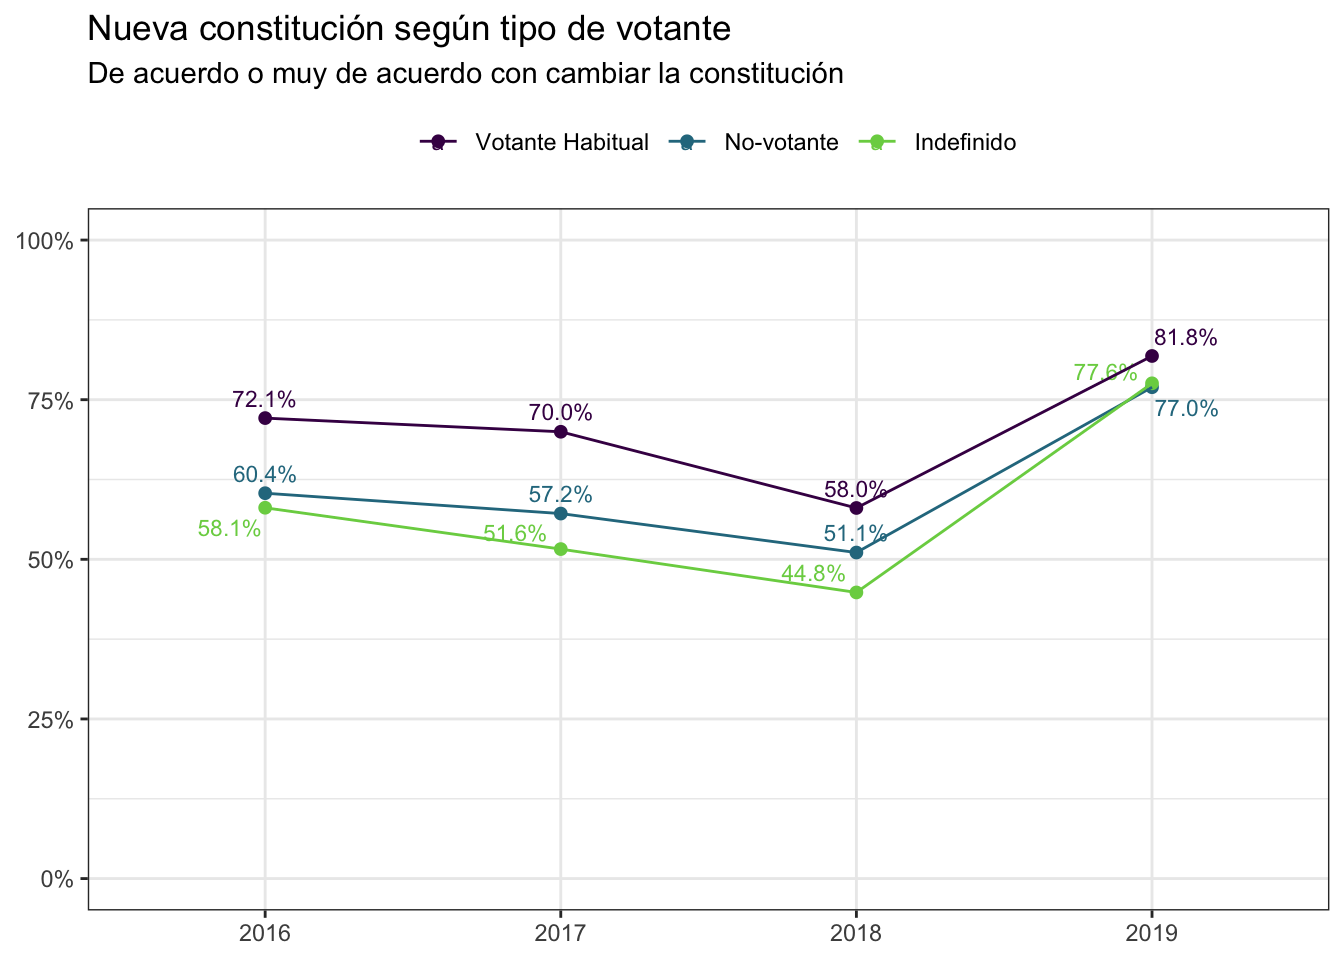
\includegraphics{reporte-elsoc_files/figure-latex/graf-consti-2-1} \end{center}

\begin{center}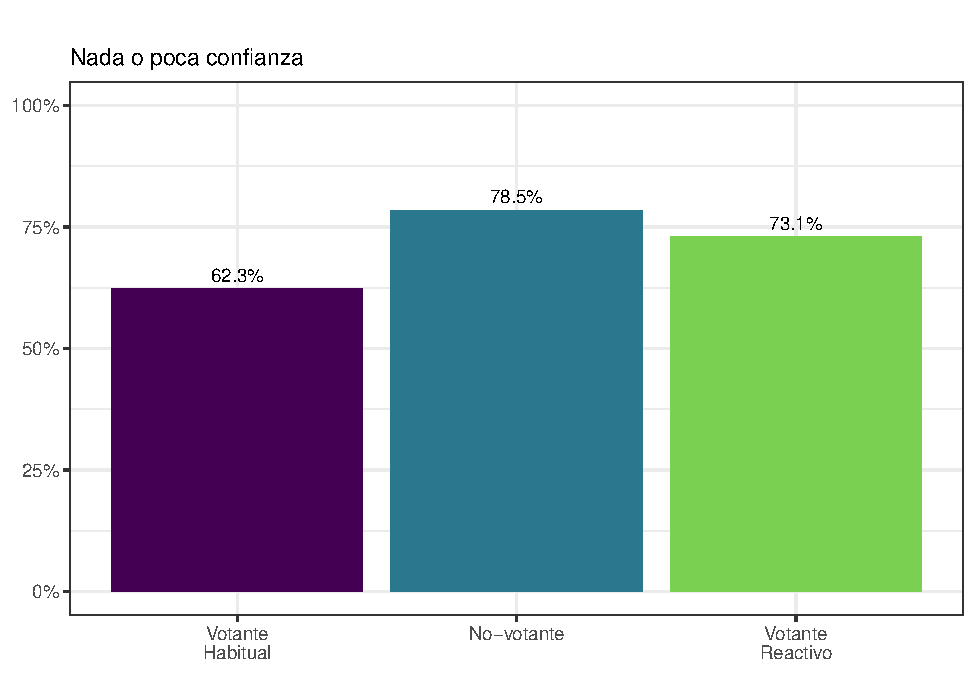
\includegraphics{reporte-elsoc_files/figure-latex/graf-convencion-2-1} \end{center}

\hypertarget{actitudes-hacia-la-democracia}{%
\section{Actitudes hacia la democracia}\label{actitudes-hacia-la-democracia}}

\begin{center}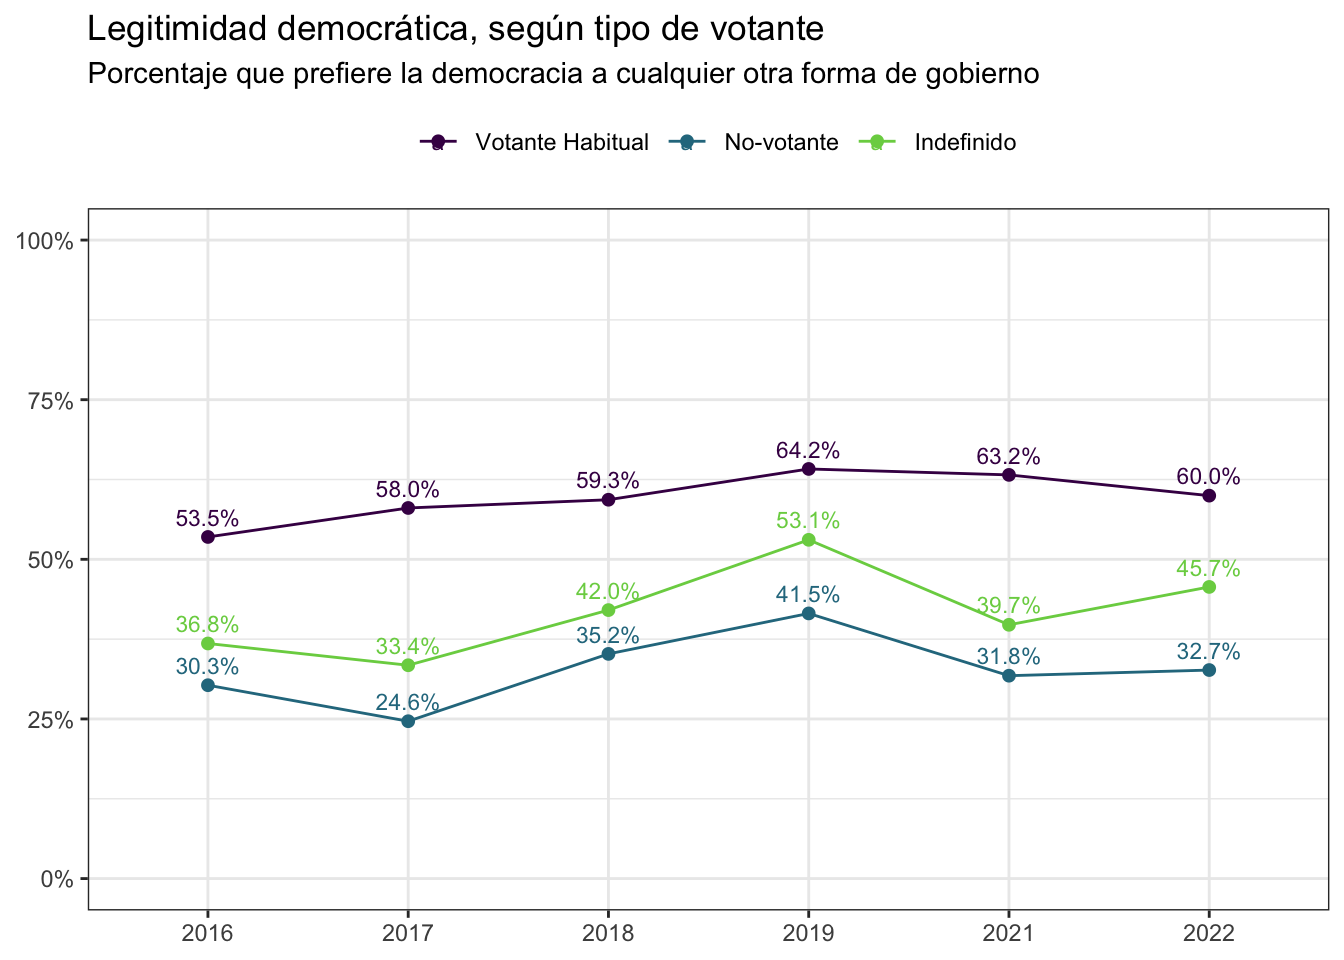
\includegraphics{reporte-elsoc_files/figure-latex/graf-leg-dem-2-1} \end{center}

\begin{center}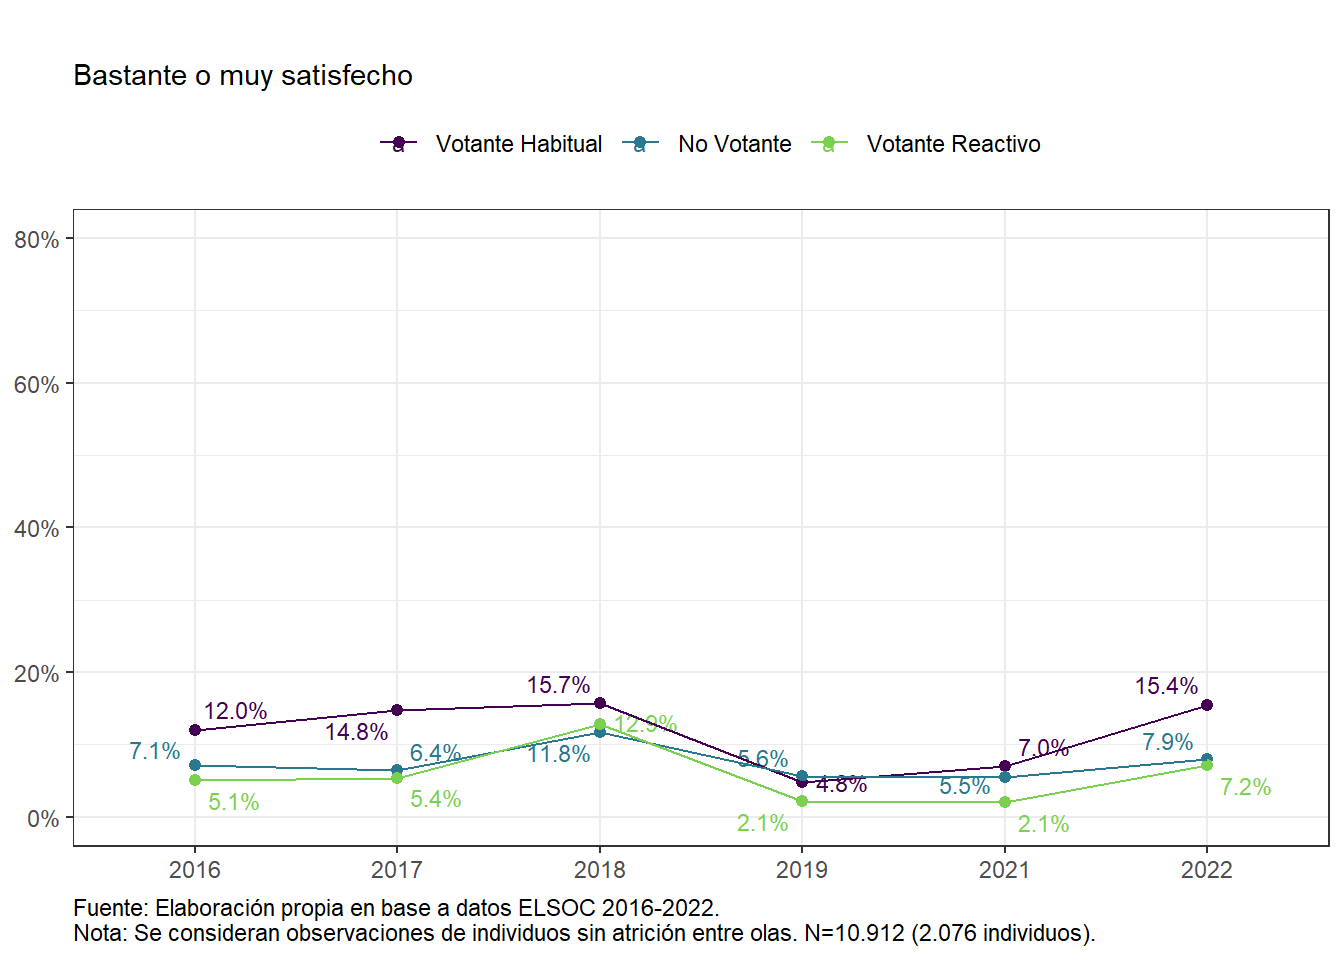
\includegraphics{reporte-elsoc_files/figure-latex/graf-satis-dem-2-1} \end{center}

\begin{center}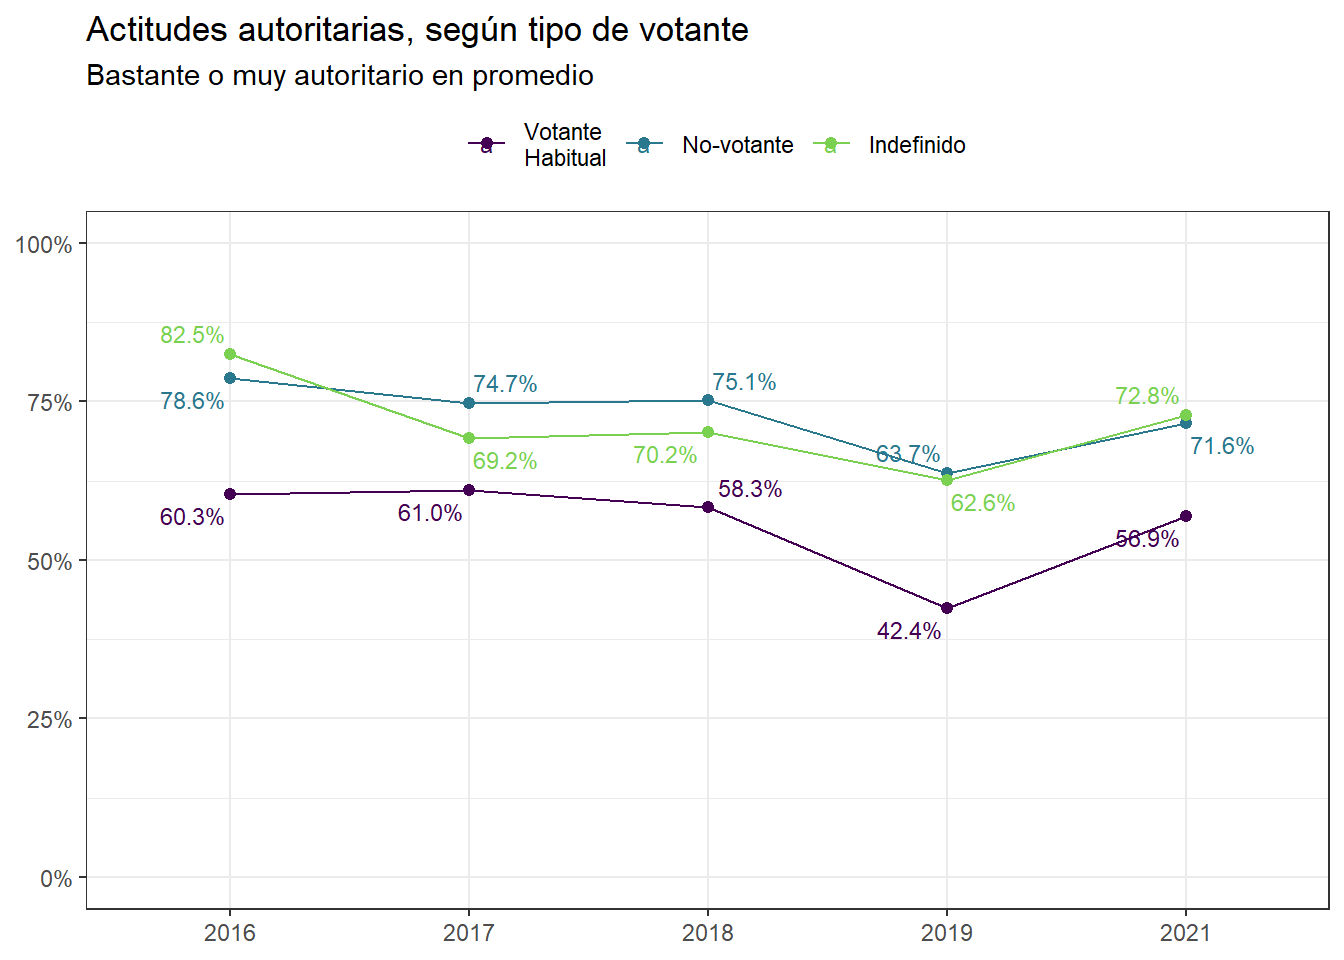
\includegraphics{reporte-elsoc_files/figure-latex/graf-autoritarismo-2-1} \end{center}

\hypertarget{identidad-e-involucramiento-poluxedtico}{%
\section{Identidad e involucramiento político}\label{identidad-e-involucramiento-poluxedtico}}

\begin{center}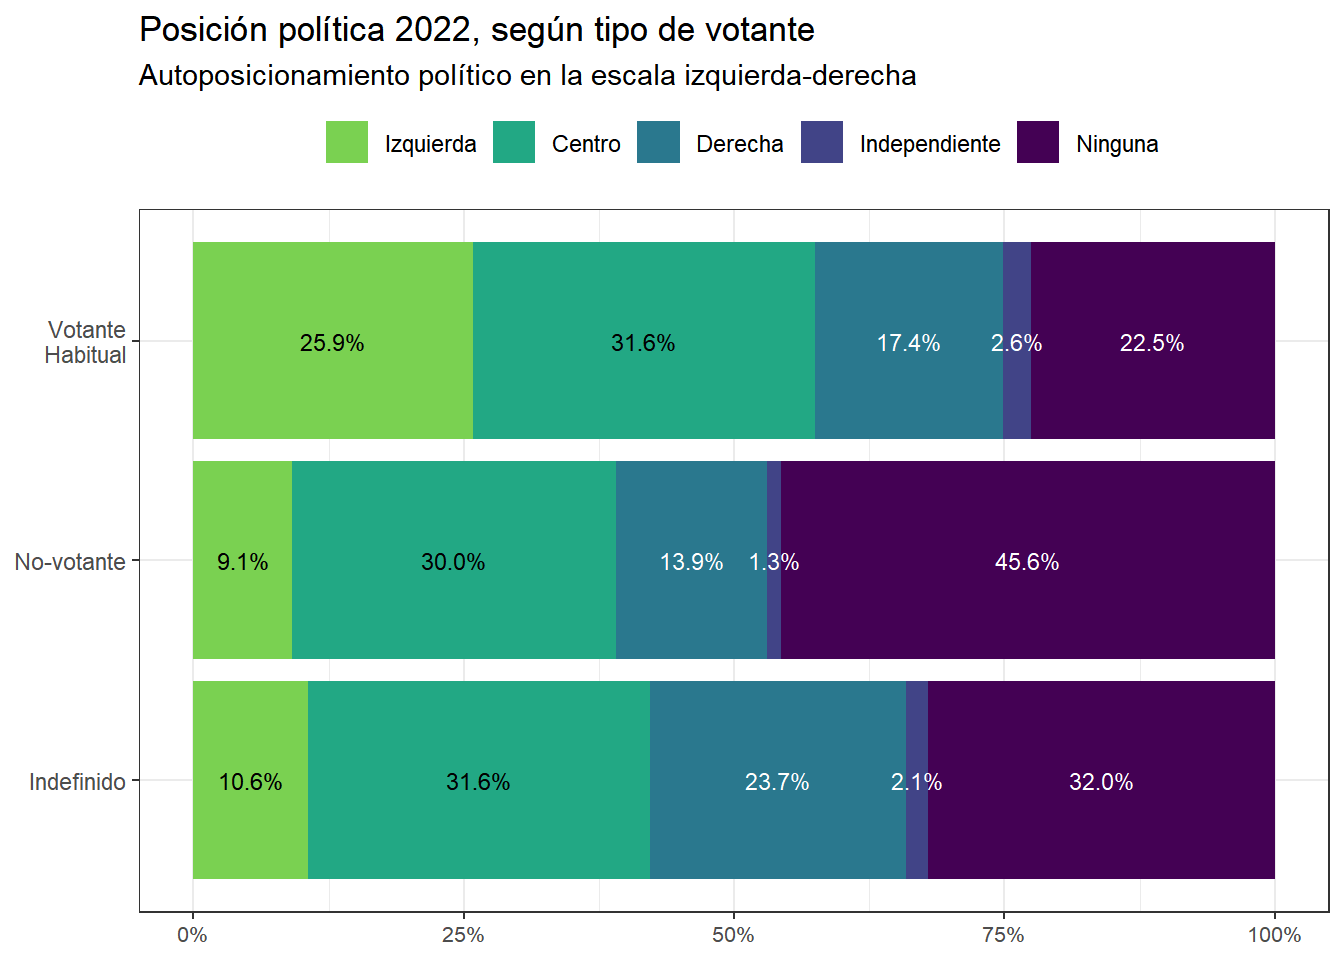
\includegraphics{reporte-elsoc_files/figure-latex/graf-posicion-pol-2-1} \end{center}

\begin{center}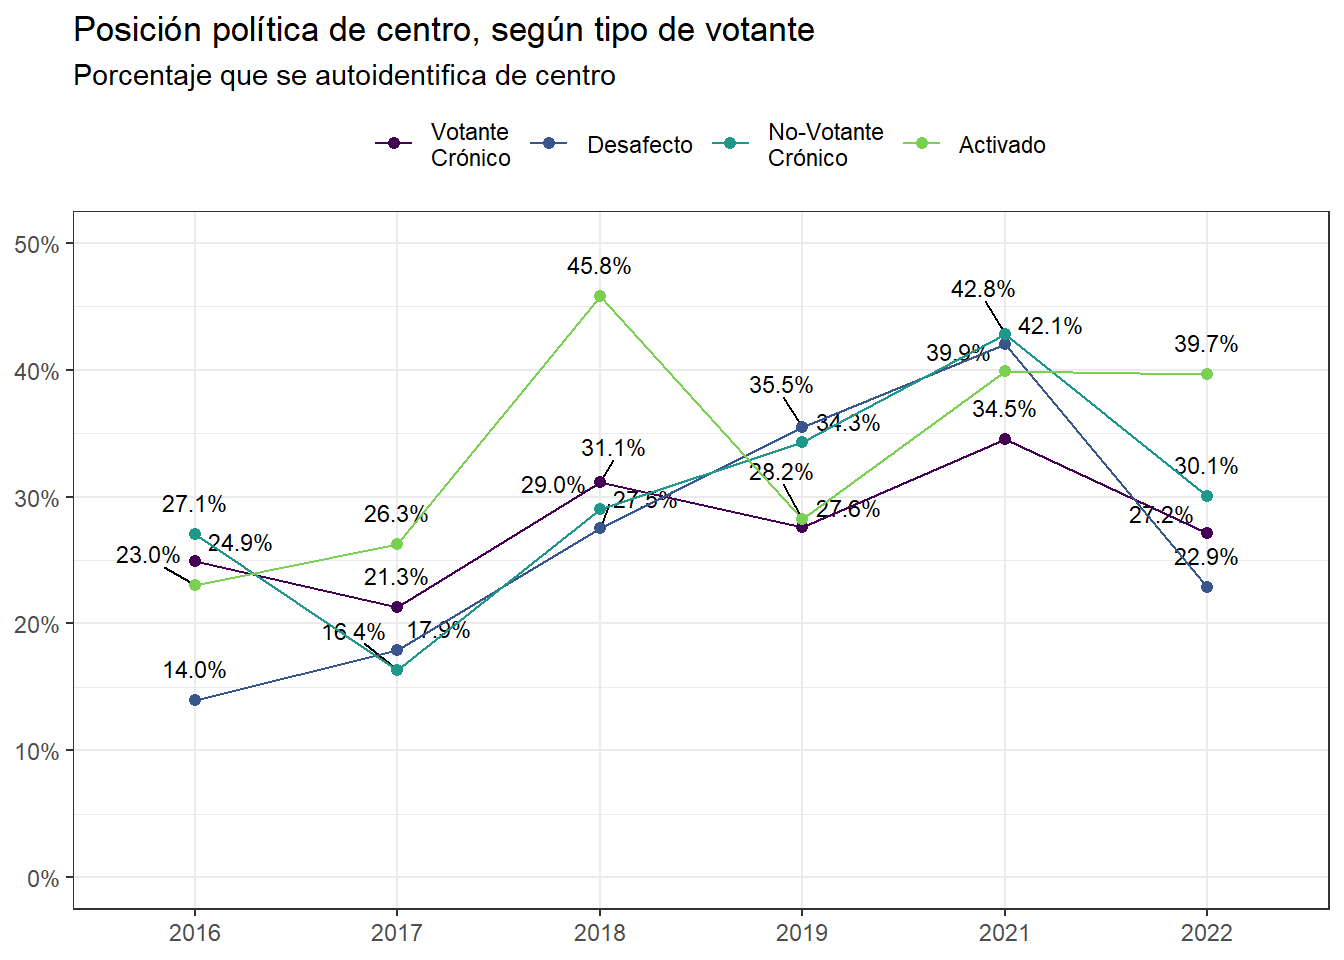
\includegraphics{reporte-elsoc_files/figure-latex/graf-centro-2-1} \end{center}

\begin{center}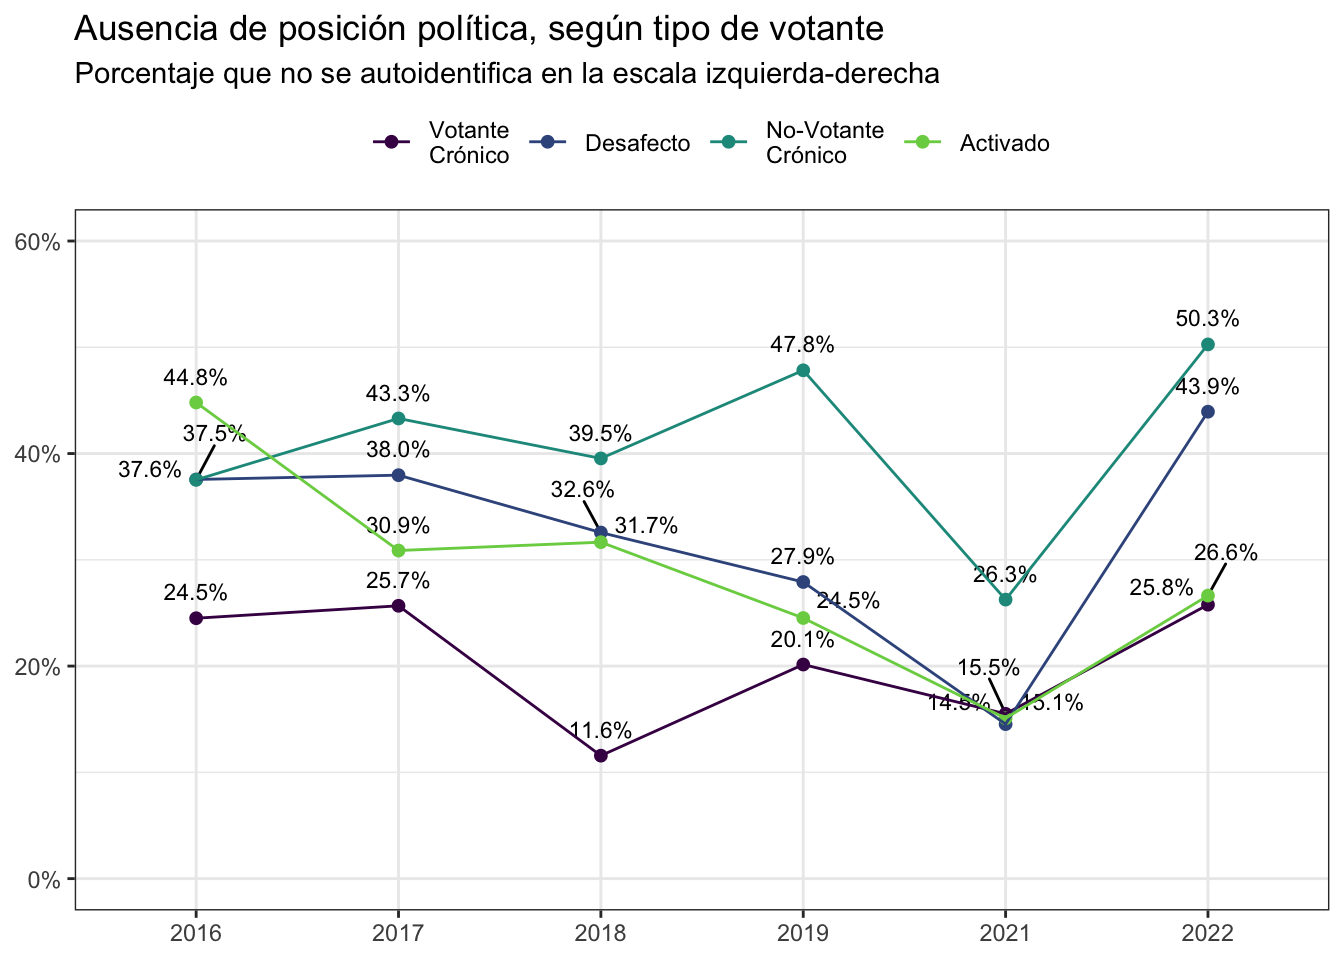
\includegraphics{reporte-elsoc_files/figure-latex/graf-sin-posicion-2-1} \end{center}

\begin{center}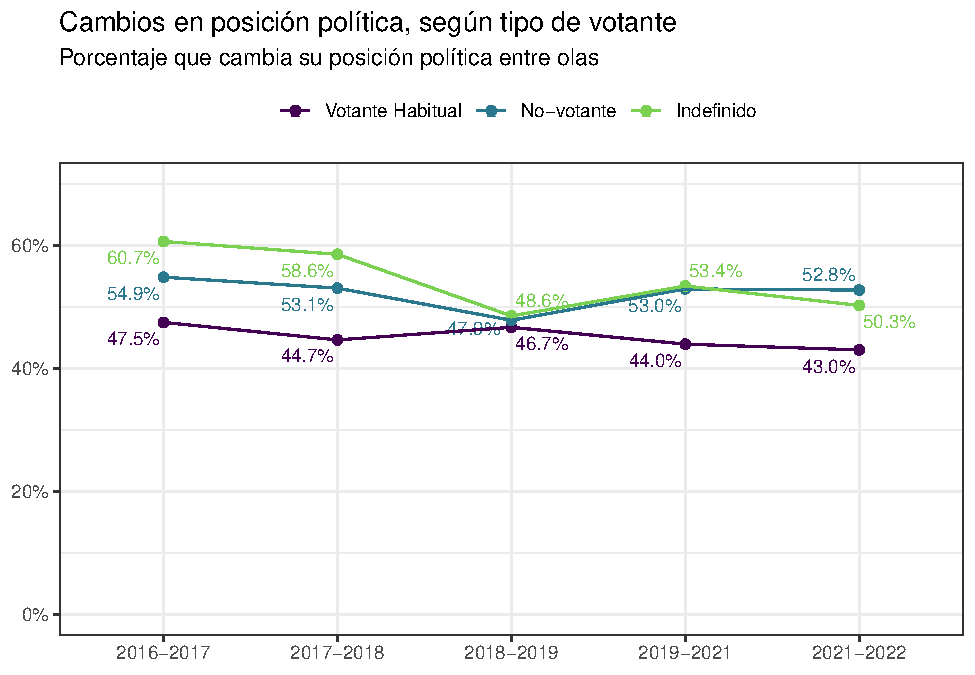
\includegraphics{reporte-elsoc_files/figure-latex/graf-cambios-idpolitica-ola-1} \end{center}

\begin{center}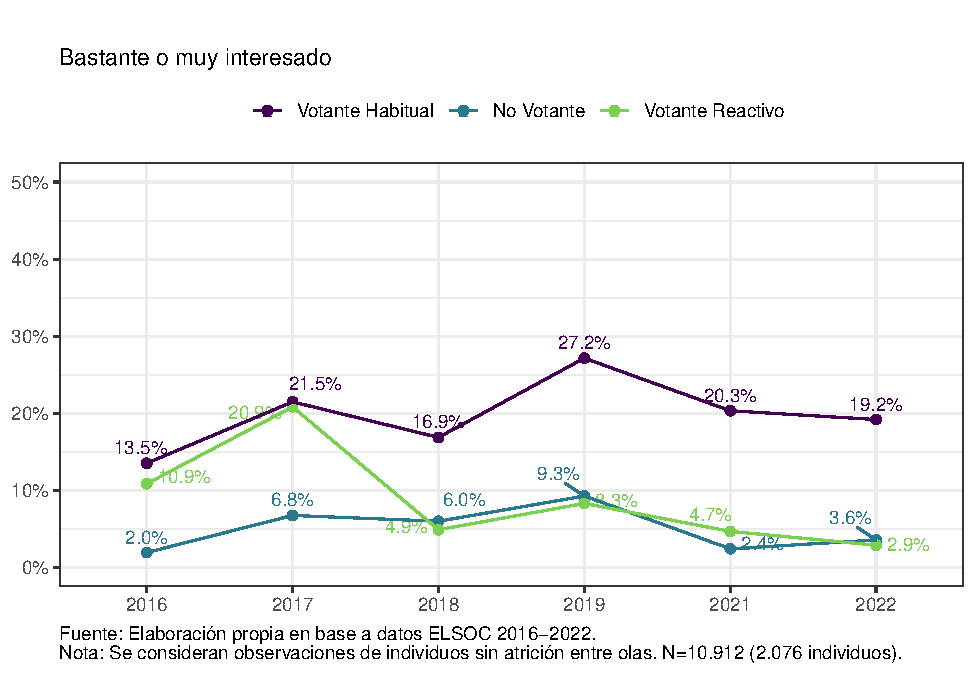
\includegraphics{reporte-elsoc_files/figure-latex/graf-interes-2-1} \end{center}

\begin{center}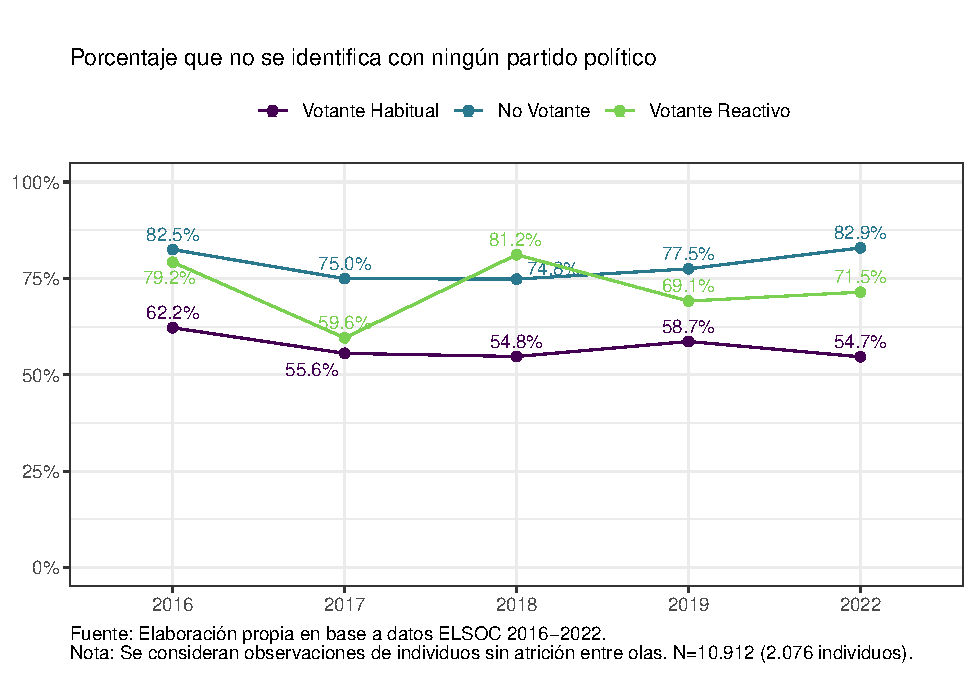
\includegraphics{reporte-elsoc_files/figure-latex/graf-id-partido-2-1} \end{center}

\begin{center}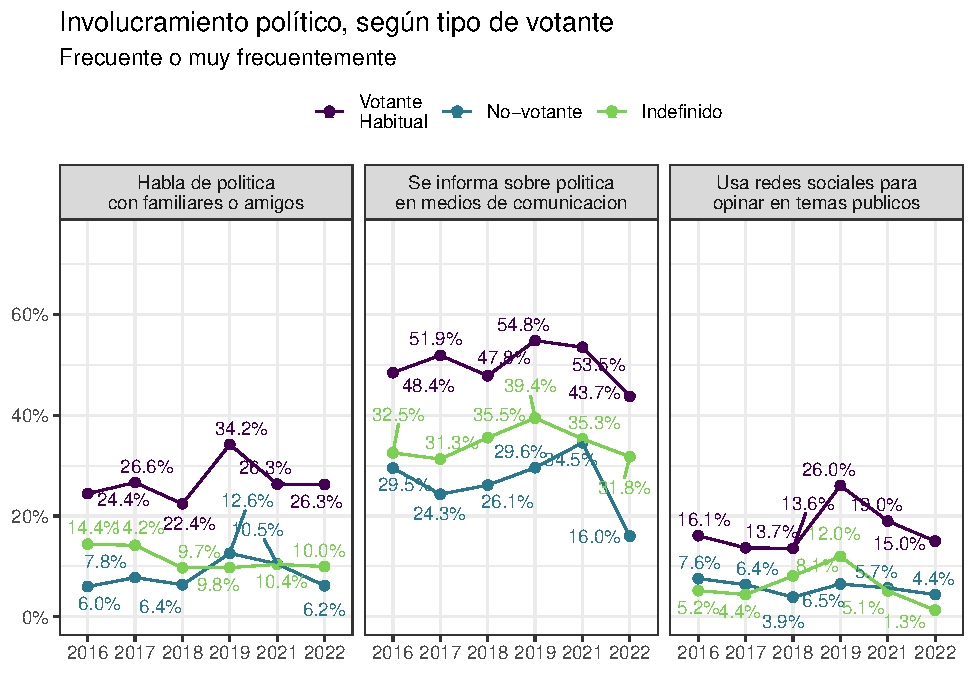
\includegraphics{reporte-elsoc_files/figure-latex/graf-involv-poli-2-1} \end{center}

\hypertarget{confianza-institucional}{%
\section{Confianza institucional}\label{confianza-institucional}}

\begin{center}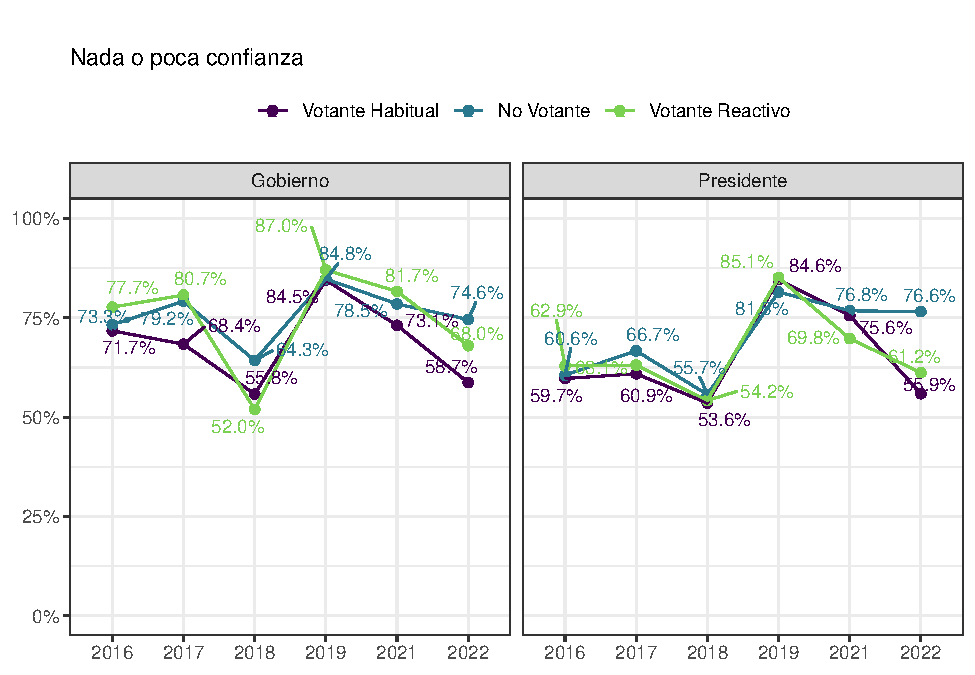
\includegraphics{reporte-elsoc_files/figure-latex/graf-conf-pol-2-1} \end{center}

\begin{center}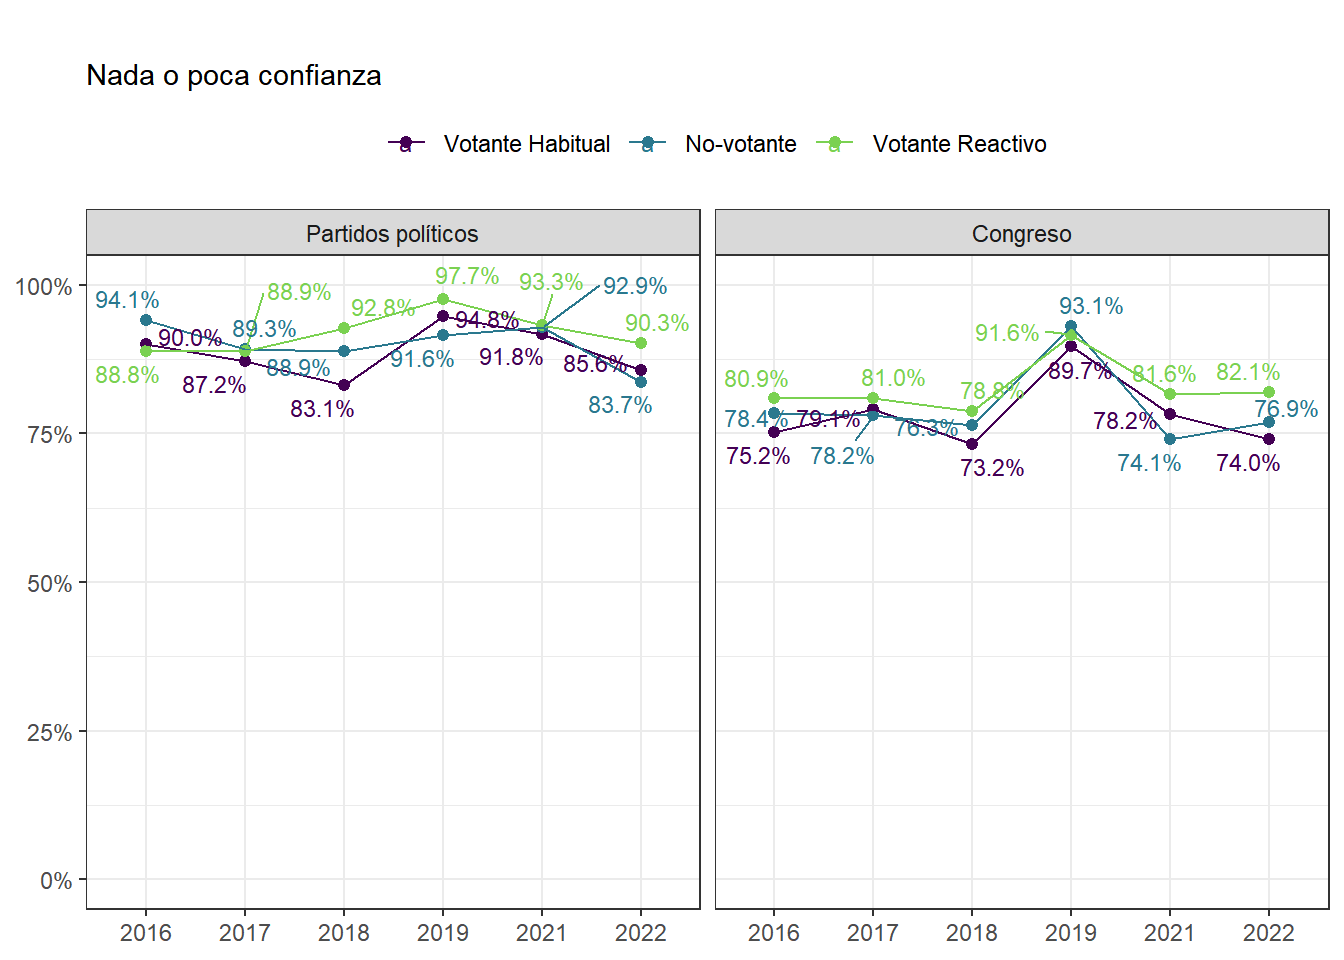
\includegraphics{reporte-elsoc_files/figure-latex/graf-conf-pol-2-2-1} \end{center}

\begin{center}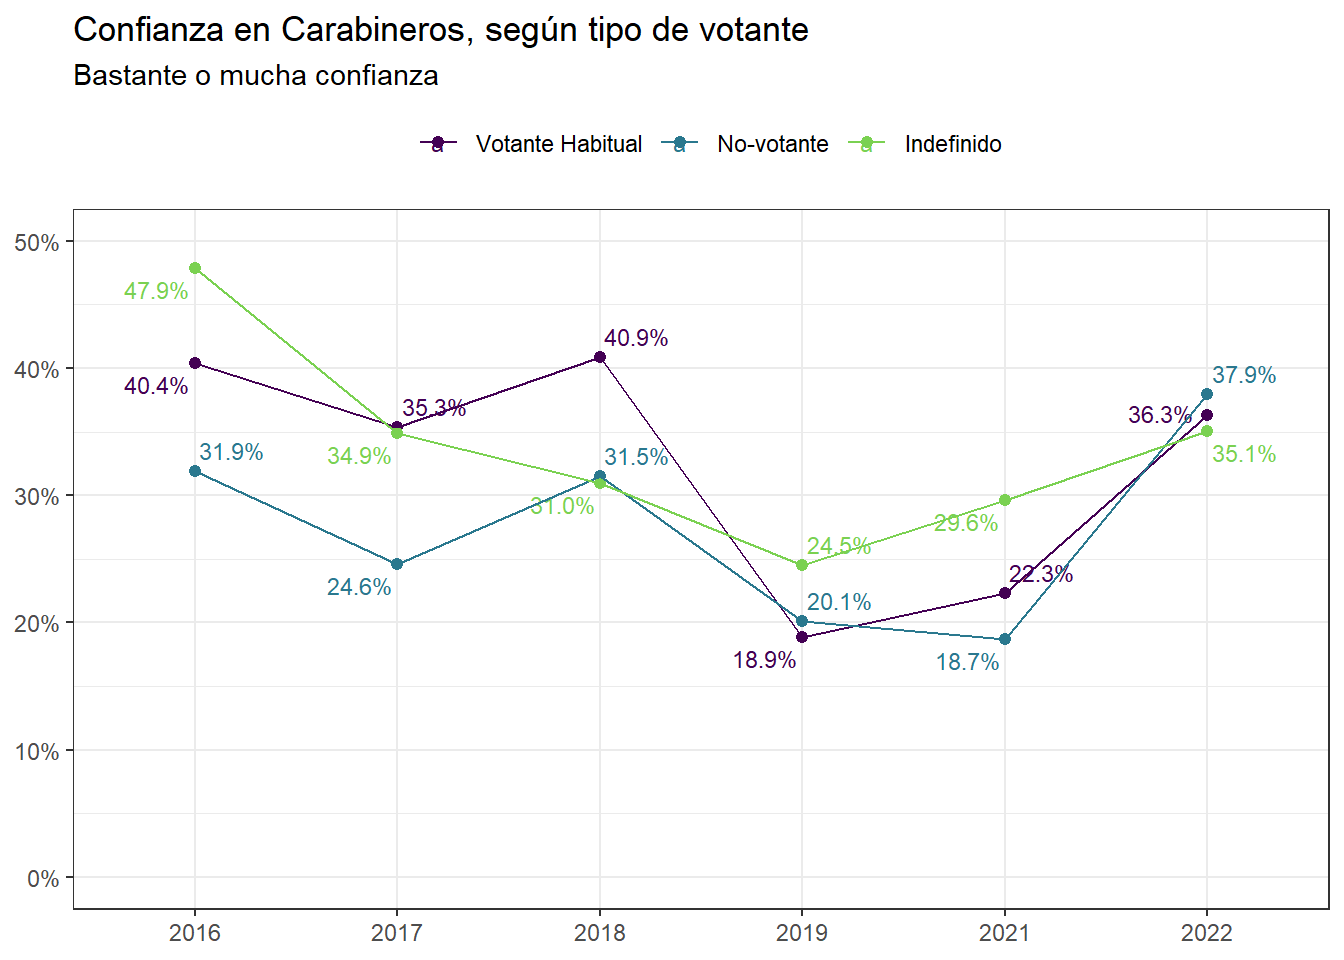
\includegraphics{reporte-elsoc_files/figure-latex/graf-carab-1} \end{center}

\hypertarget{movilizaciuxf3n-social}{%
\section{Movilización social}\label{movilizaciuxf3n-social}}

\begin{center}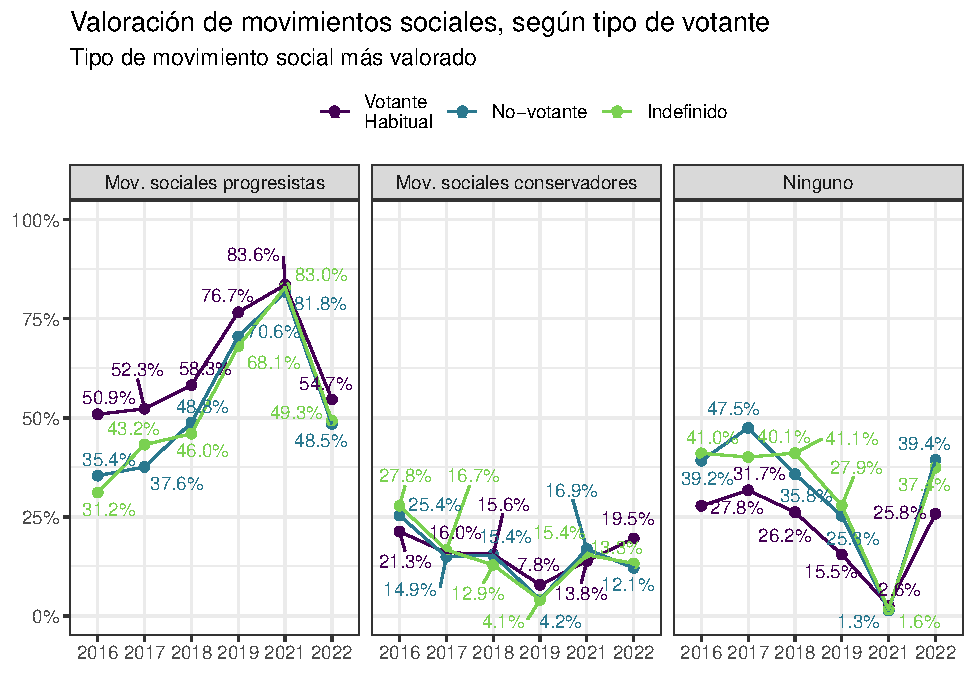
\includegraphics{reporte-elsoc_files/figure-latex/graf-mov-tipo-2-1} \end{center}

\begin{center}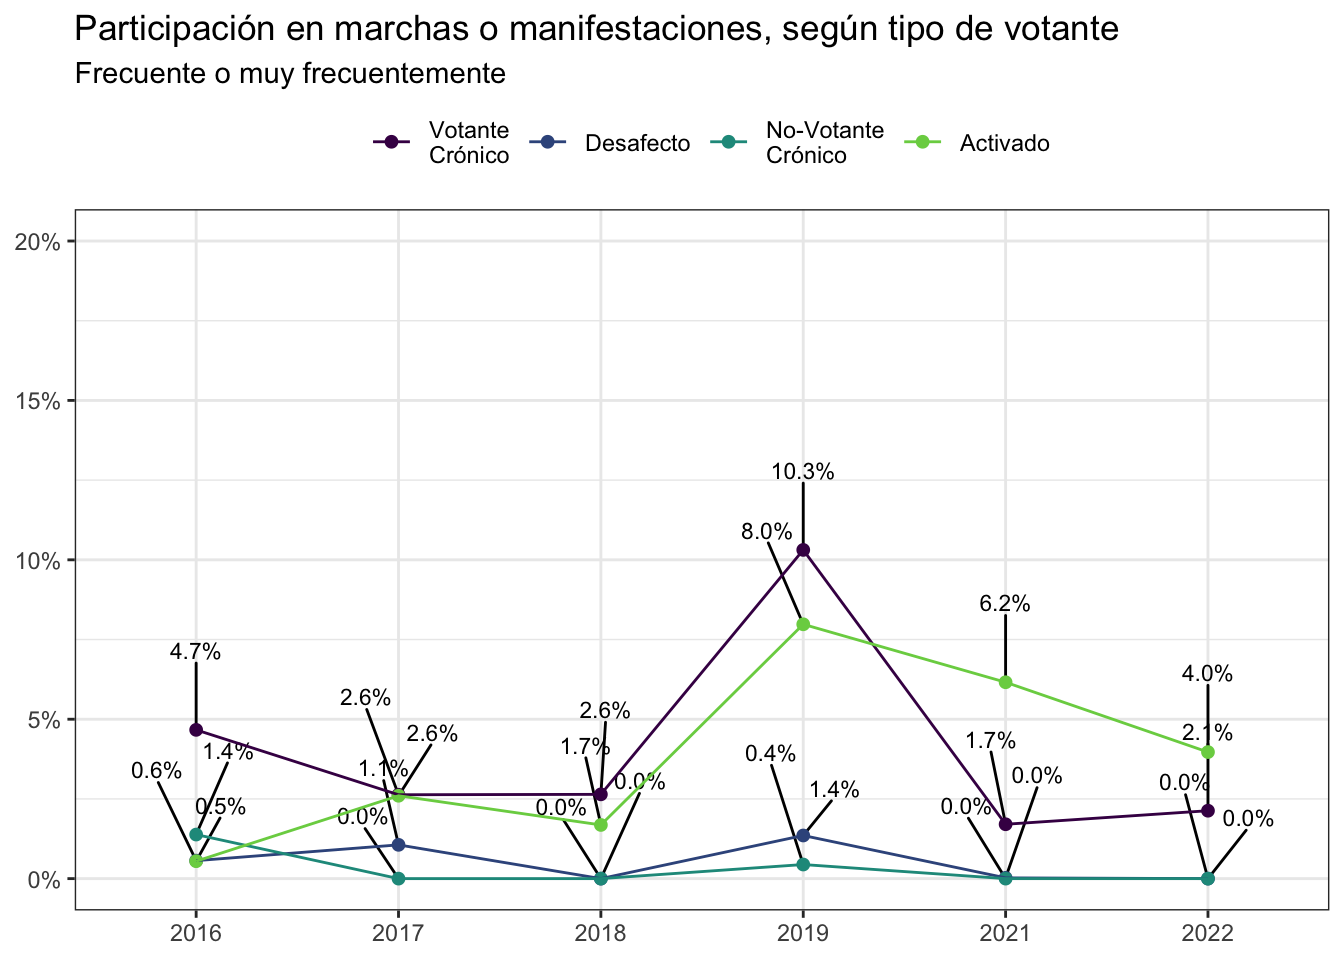
\includegraphics{reporte-elsoc_files/figure-latex/graf-parti-mov-2-1} \end{center}

\hypertarget{opiniuxf3n-puxfablica-y-contingencia}{%
\section{Opinión pública y contingencia}\label{opiniuxf3n-puxfablica-y-contingencia}}

\begin{center}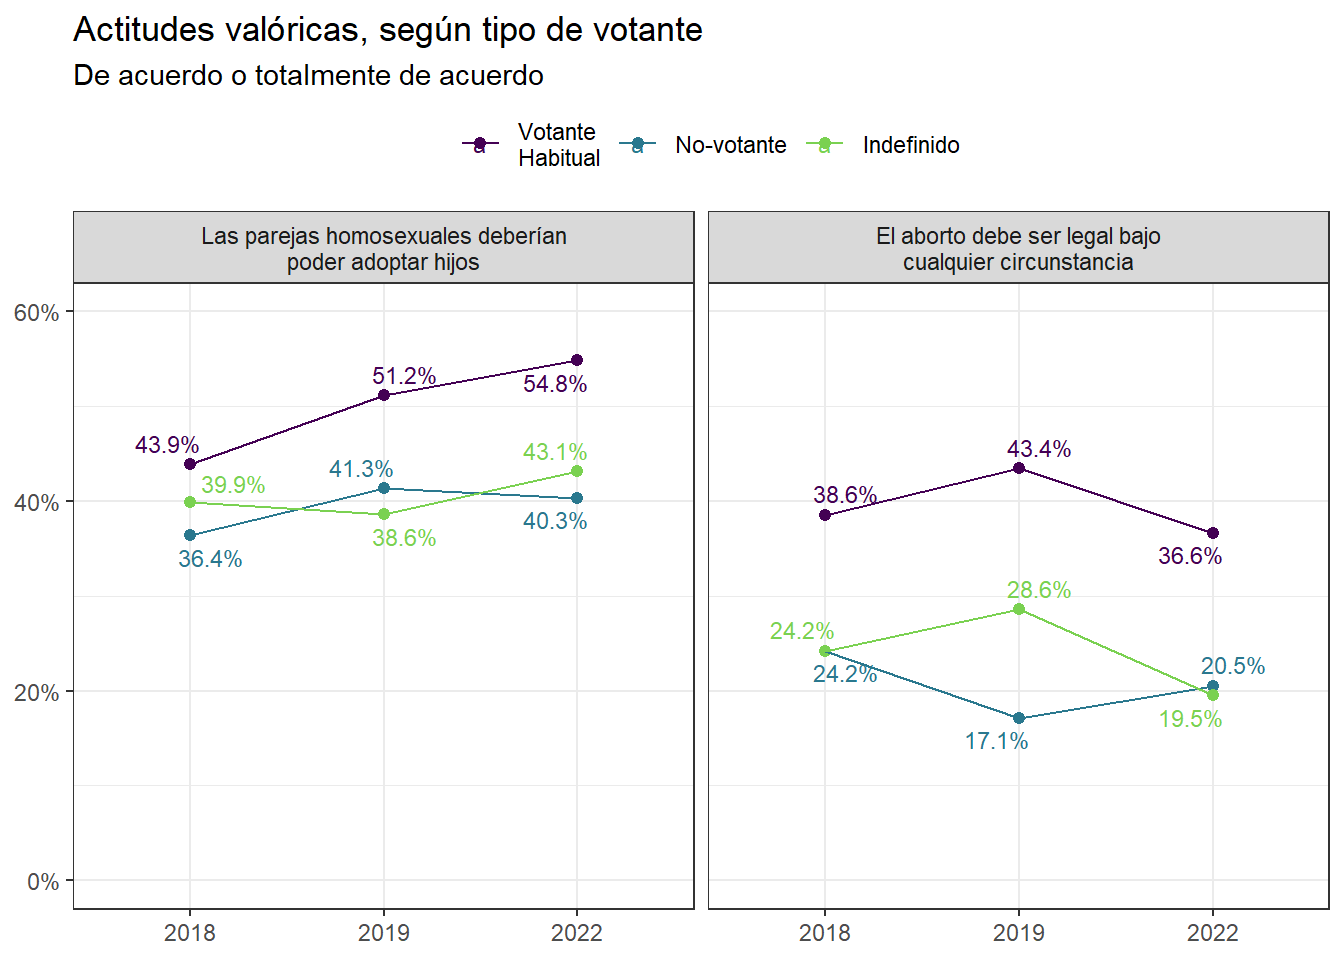
\includegraphics{reporte-elsoc_files/figure-latex/graf-op-valores-2-1} \end{center}

\begin{center}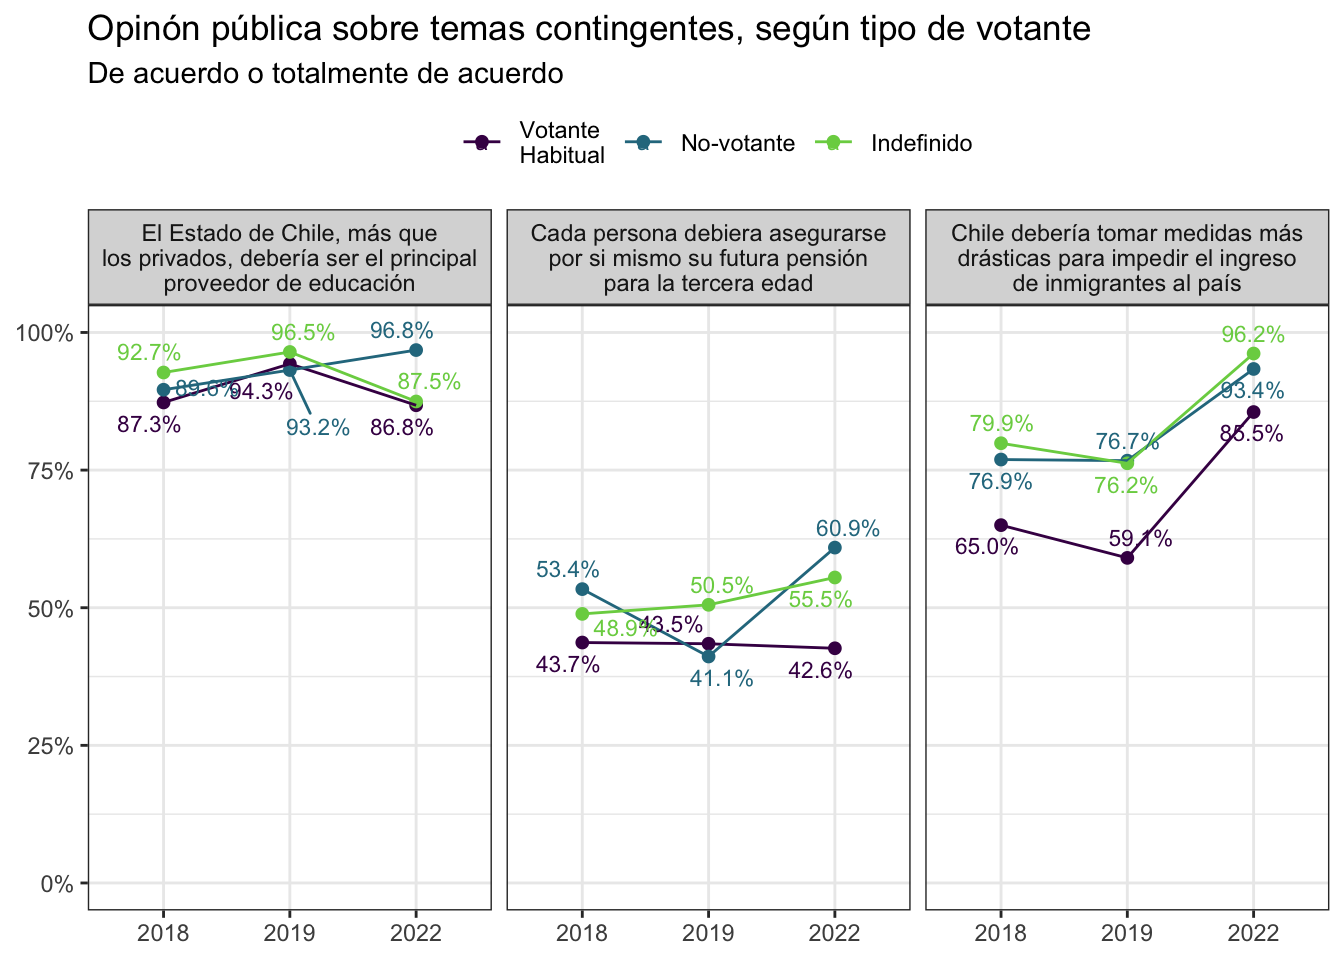
\includegraphics{reporte-elsoc_files/figure-latex/graf-op-contingente-2-1} \end{center}

\begin{center}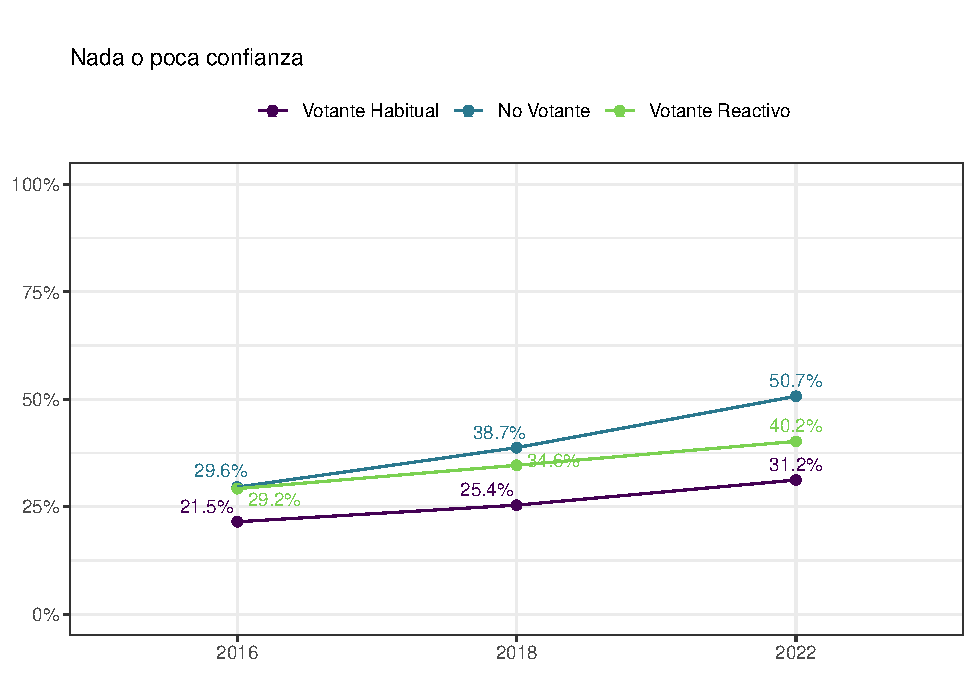
\includegraphics{reporte-elsoc_files/figure-latex/desconf-mapuche-1} \end{center}

\begin{center}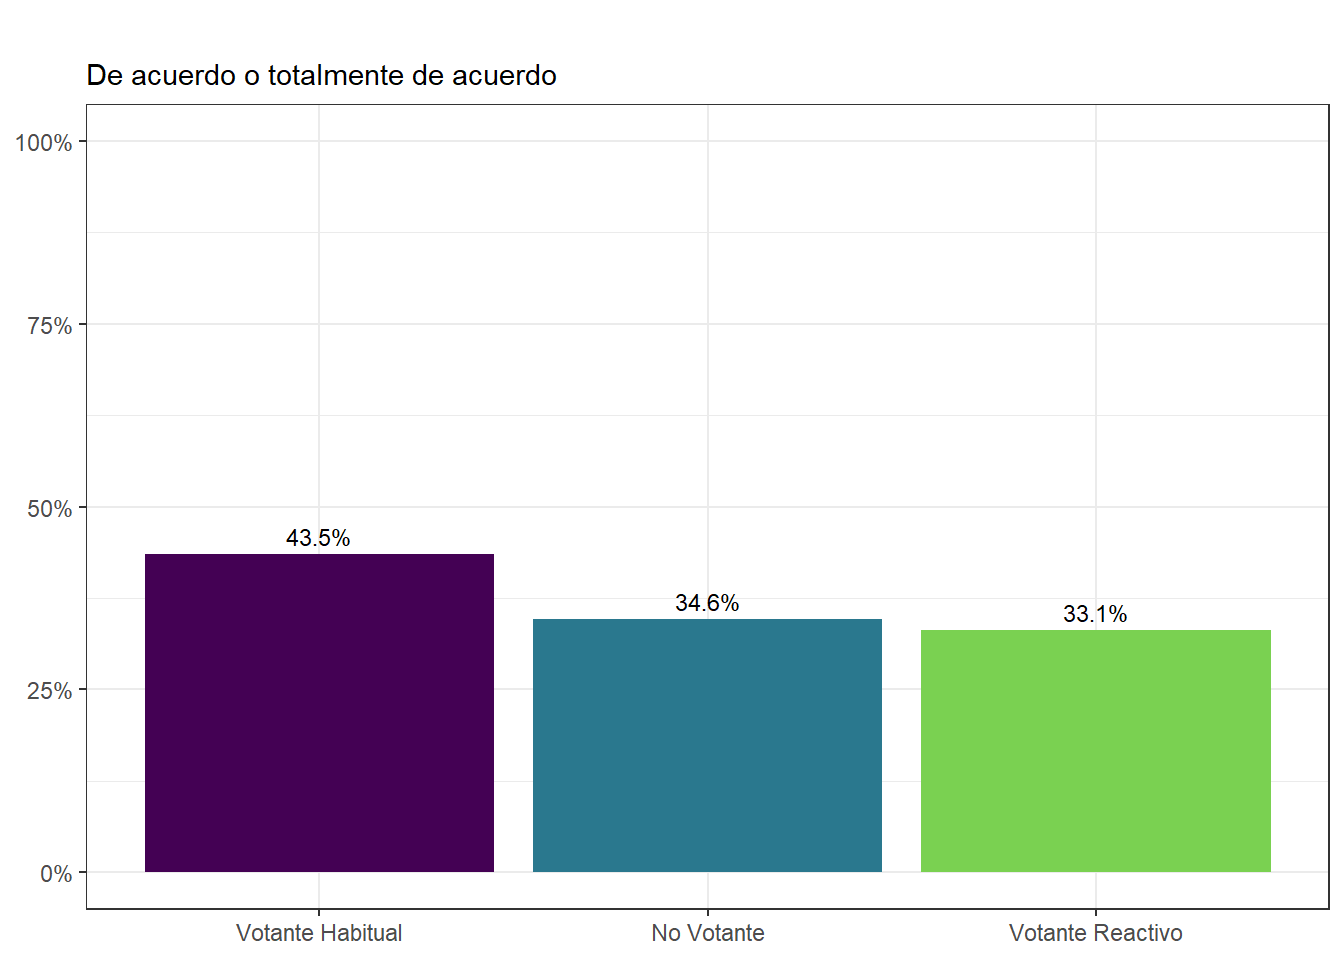
\includegraphics{reporte-elsoc_files/figure-latex/consti-mapuche-1} \end{center}

\begin{center}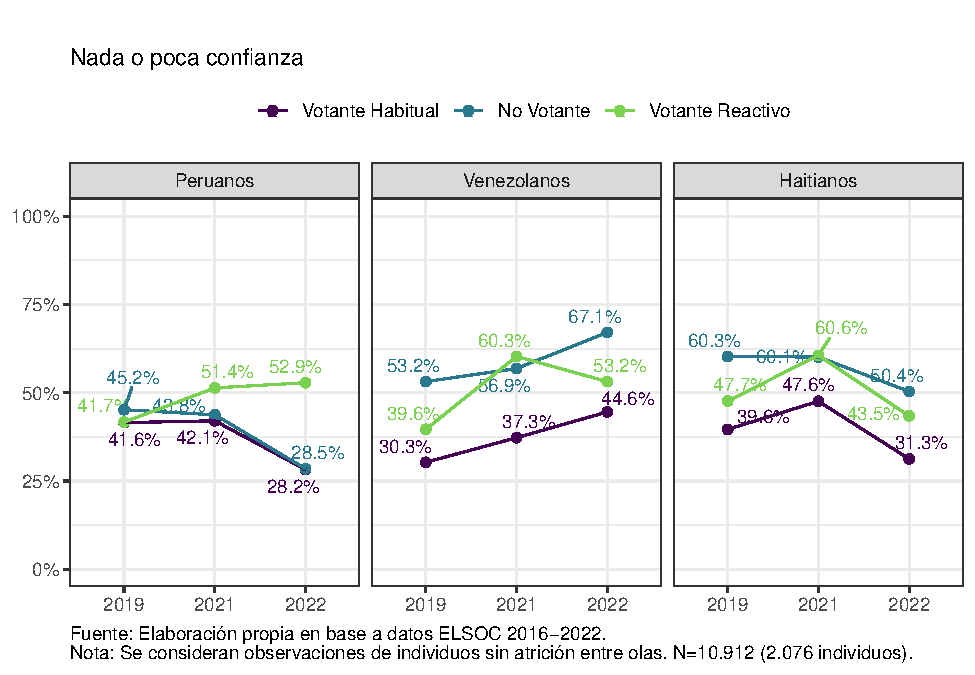
\includegraphics{reporte-elsoc_files/figure-latex/desconf-inmigrante-1} \end{center}

\begin{center}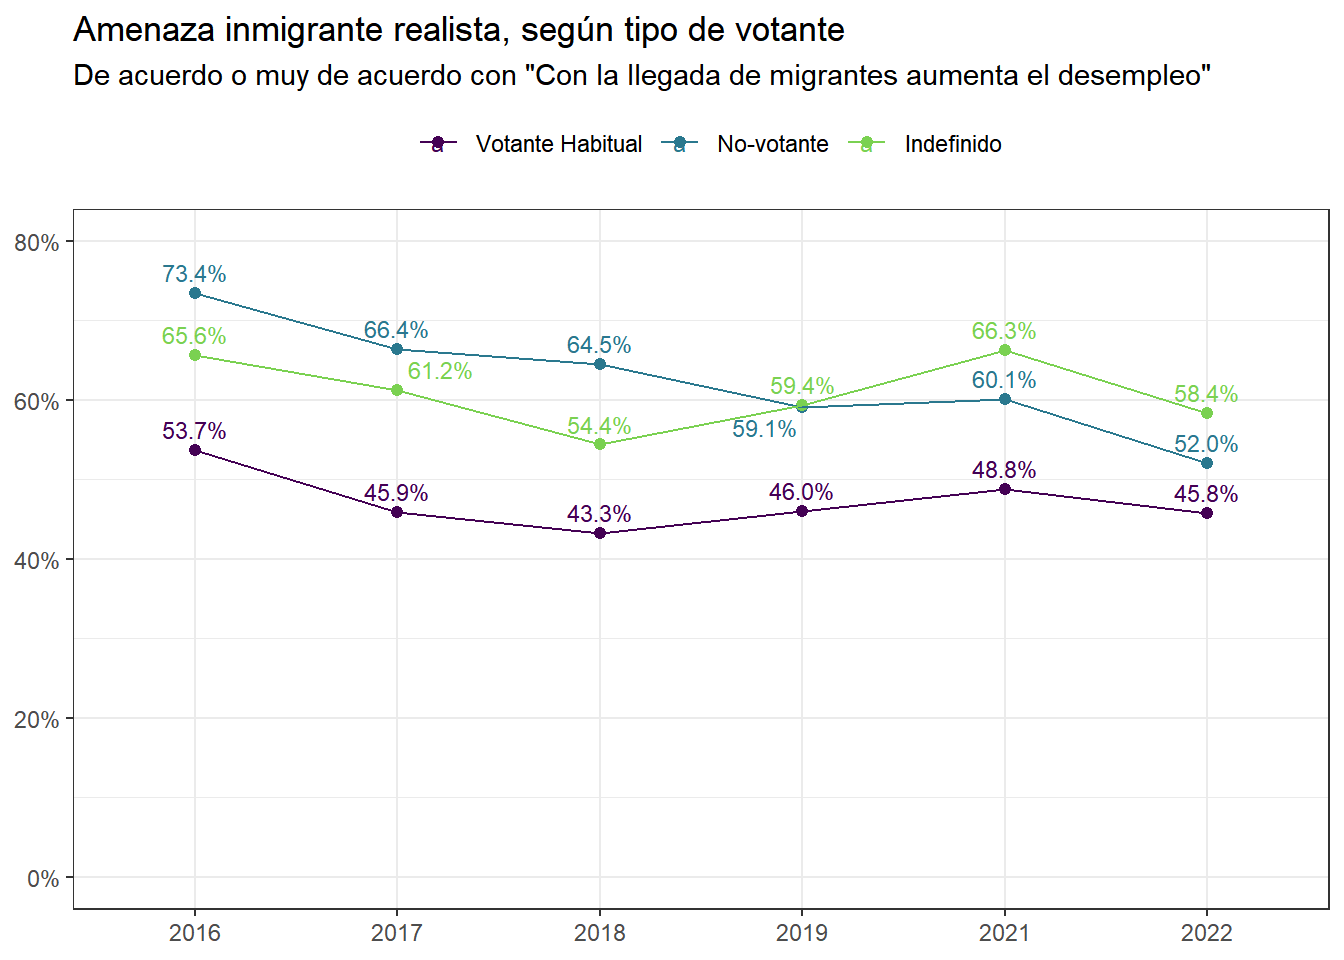
\includegraphics{reporte-elsoc_files/figure-latex/ame-realista-1} \end{center}

\begin{center}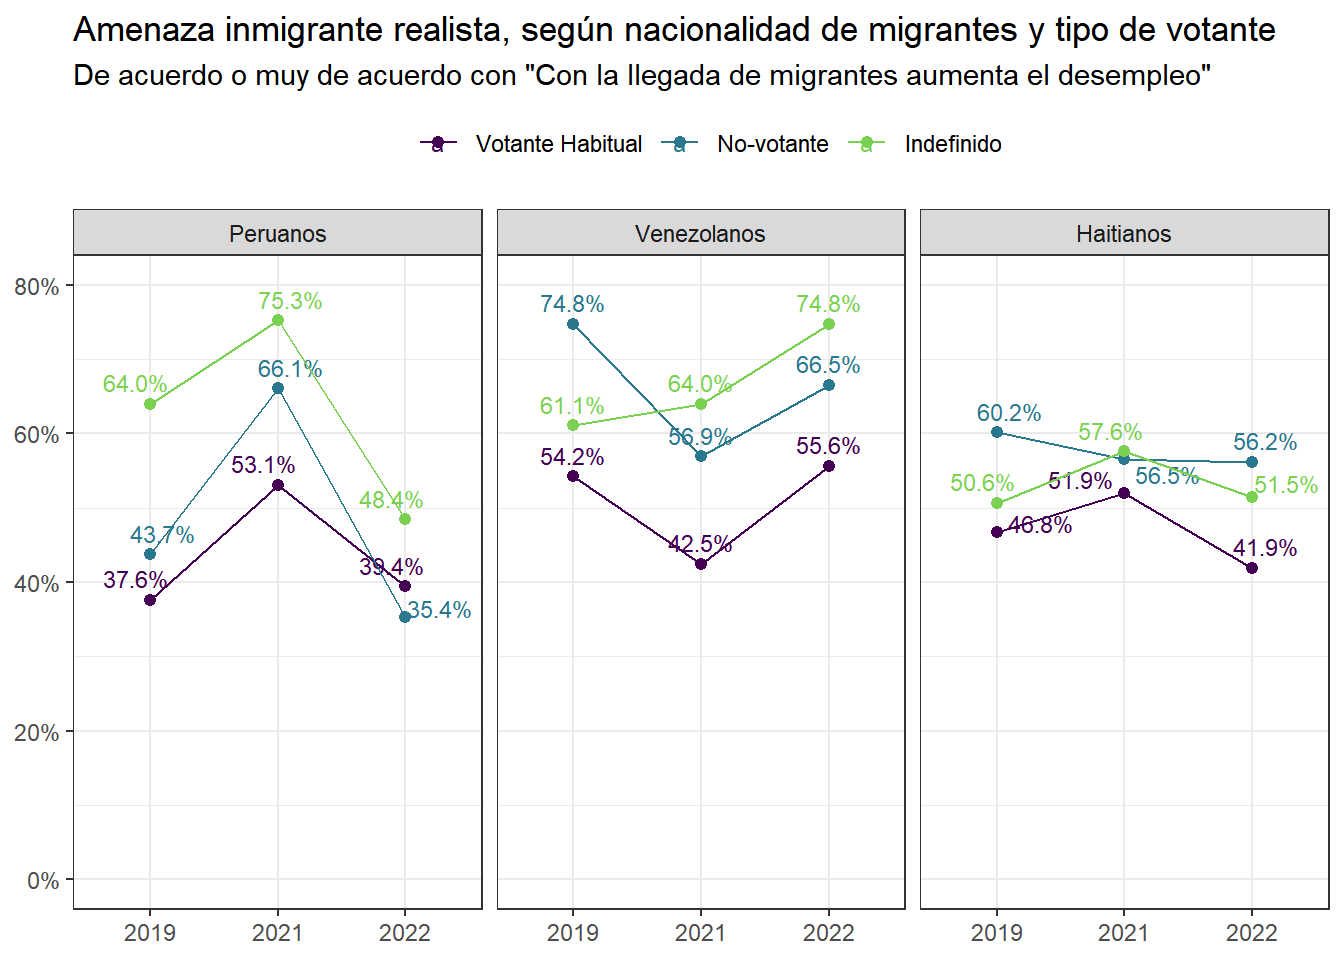
\includegraphics{reporte-elsoc_files/figure-latex/ame-realista-proced-1} \end{center}

\begin{center}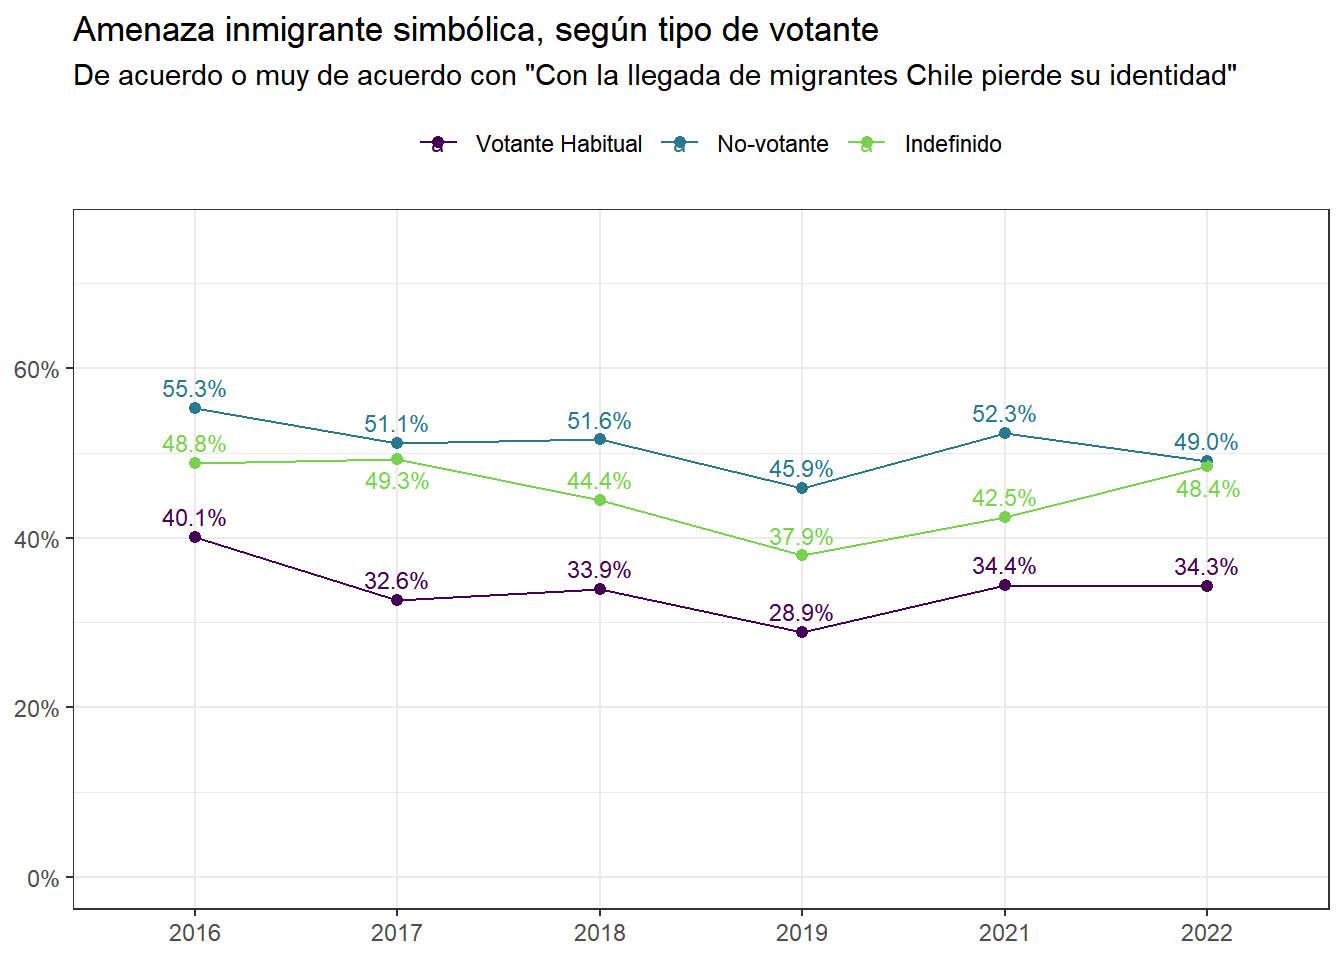
\includegraphics{reporte-elsoc_files/figure-latex/ame-simbolica-1} \end{center}

\begin{center}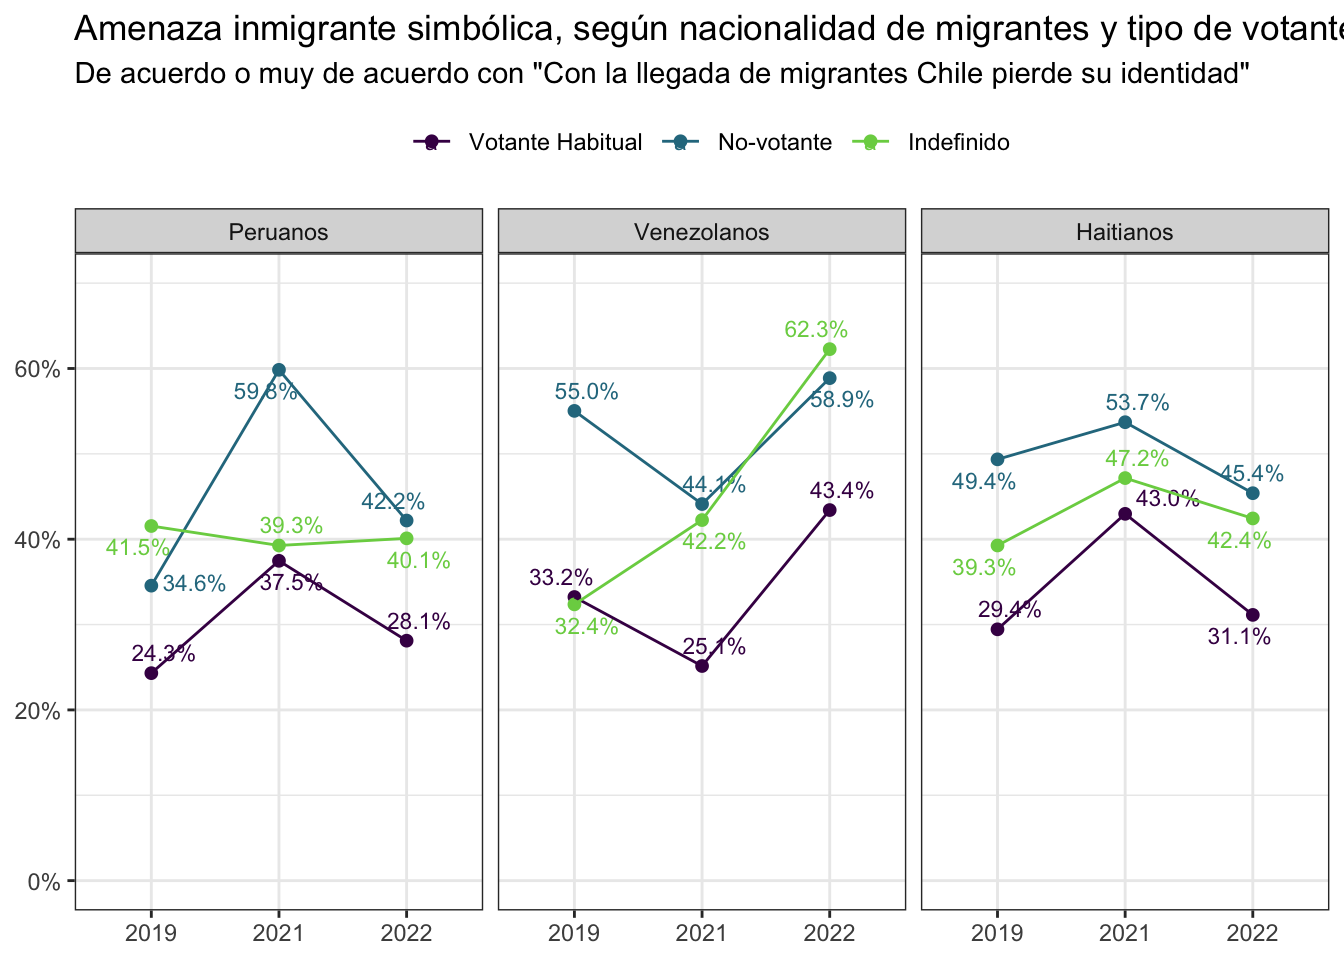
\includegraphics{reporte-elsoc_files/figure-latex/ame-simbolica-proced-1} \end{center}

\hypertarget{justificaciuxf3n-de-la-violencia}{%
\section{Justificación de la violencia}\label{justificaciuxf3n-de-la-violencia}}

\begin{center}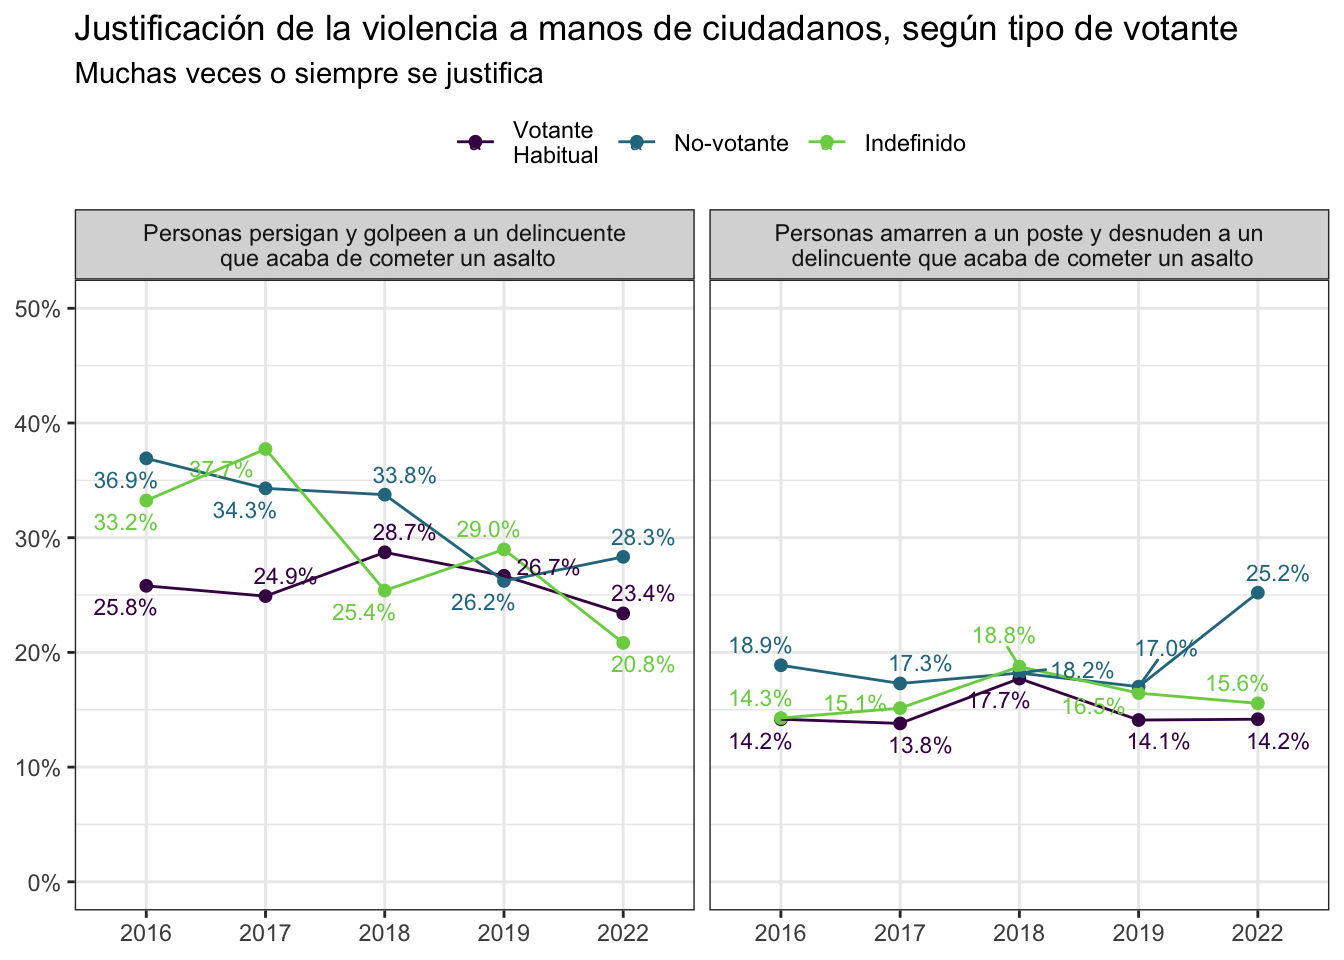
\includegraphics{reporte-elsoc_files/figure-latex/graf-justviolencia1-ola-2-1} \end{center}

\begin{center}\includegraphics{reporte-elsoc_files/figure-latex/graf-justviolencia2-ola-2-1} \end{center}

\hypertarget{cohesiuxf3n-social}{%
\chapter{Cohesión social}\label{cohesiuxf3n-social}}

\hypertarget{calidad-del-vuxednculo-social}{%
\section{Calidad del vínculo social:}\label{calidad-del-vuxednculo-social}}

\begin{center}\includegraphics{reporte-elsoc_files/figure-latex/unnamed-chunk-1-1} \end{center}

\begin{center}\includegraphics{reporte-elsoc_files/figure-latex/indice-diversidad-part-1} \end{center}

\hypertarget{sentido-de-pertenencia}{%
\section{Sentido de pertenencia}\label{sentido-de-pertenencia}}

\begin{center}\includegraphics{reporte-elsoc_files/figure-latex/graf-orgullochileno-perfil-1} \end{center}

\hypertarget{percepciuxf3n-de-justicia}{%
\subsection{Percepción de justicia}\label{percepciuxf3n-de-justicia}}

\begin{center}\includegraphics{reporte-elsoc_files/figure-latex/indice-percjusticia-part-1} \end{center}

\hypertarget{vuxednculos-territoriales}{%
\section{Vínculos Territoriales}\label{vuxednculos-territoriales}}

\begin{center}\includegraphics{reporte-elsoc_files/figure-latex/unnamed-chunk-2-1} \end{center}

\begin{center}\includegraphics{reporte-elsoc_files/figure-latex/confli-olas-part-1} \end{center}

\begin{center}\includegraphics{reporte-elsoc_files/figure-latex/crim-olas-part-1} \end{center}

\begin{center}\includegraphics{reporte-elsoc_files/figure-latex/inseg-part-1} \end{center}

\hypertarget{bienestar}{%
\section{Bienestar}\label{bienestar}}

\hypertarget{satisfacciuxf3n-vital}{%
\subsection{Satisfacción vital}\label{satisfacciuxf3n-vital}}

\begin{center}\includegraphics{reporte-elsoc_files/figure-latex/unnamed-chunk-3-1} \end{center}

\hypertarget{carga-econuxf3mica}{%
\subsection{Carga económica}\label{carga-econuxf3mica}}

\begin{center}\includegraphics{reporte-elsoc_files/figure-latex/unnamed-chunk-4-1} \end{center}

\hypertarget{movilidad-social}{%
\subsection{Movilidad social}\label{movilidad-social}}

\begin{center}\includegraphics{reporte-elsoc_files/figure-latex/unnamed-chunk-5-1} \end{center}

\end{document}
